\documentclass[12pt]{ociamthesis}  % default square logo 
%\documentclass[12pt,beltcrest]{ociamthesis} % use old belt crest logo
%\documentclass[12pt,shieldcrest]{ociamthesis} % use older shield crest logo

%load any additional packages
\usepackage[utf8]{inputenc}
\usepackage{amsmath}
\usepackage{amsfonts}
\usepackage{amssymb}
\usepackage{graphicx}
\usepackage{subcaption}
\usepackage{epstopdf}
\usepackage{msc}

%input macros (i.e. write your own macros file called mymacros.tex 
%and uncomment the next line)
%\include{mymacros}

\title{Secure Protocol for  \\[1ex]
       Courier-Dependent \\[1ex]
       Communication}   %note \\[1ex] is a line break in the title

\author{Chen Sun}             %your name
\college{Trinity College}  %your college

%\renewcommand{\submittedtext}{change the default text here if needed}
\degree{Master of Science}     %the degree
\degreedate{Trinity 2014}         %the degree date

%end the preamble and start the document
\begin{document}

%this baselineskip gives sufficient line spacing for an examiner to easily
%markup the thesis with comments
\baselineskip=18pt plus1pt

%set the number of sectioning levels that get number and appear in the contents
\setcounter{secnumdepth}{3}
\setcounter{tocdepth}{3}


\maketitle                  % create a title page from the preamble info
%\begin{dedication}
This thesis is dedicated to\\
 someone\\
for some special reason\\
\end{dedication}        % include a dedication.tex file
\begin{acknowledgements}
plenty of waffle, plenty of waffle, plenty of waffle, plenty of waffle,
plenty of waffle, plenty of waffle, plenty of waffle, plenty of waffle.
\end{acknowledgements}   % include an acknowledgements.tex file
\begin{abstract}
On the contrary of modern Internet - which provides reliable and continuous connection between end-to-end users, the so called ``challenged networks" denotes a group of networks which are characterized by high latency, restricted bandwidth limitation, short node longevity or bad path stability. In those challenged networks, typical TCP/IP protocol will not be functioning any more, thus other ways have to be used to establish connections within these networks. One of the common methods to achieve communication within challenged networks appears to be using portable devices as couriers to deliver the message for end users. Although this method has been widely used, it is spotted that this intuitive method leaks the information about communication content thus extra work need to be done to ensure its secure communication.
\\

To solve the problem, this thesis aims to create a new protocol to allow secure and efficient communication established in the courier-dependent networks. In this these, first it formalizes such courier-dependent communications by creating a specific communication scenario which takes its security properties into account. Then it proposes a secure protocol for the specific scenario. The protocol provides mainly 4 security guarantees during the communication - authentication, authenticity of origin, confidentiality and deniability. After that, an application of the protocol is developed and the evaluation of the application proves its efficiency and scalability meets the general requirement as an applicable implementation.
\end{abstract}          % include the abstract

\begin{romanpages}          % start roman page numbering
\tableofcontents            % generate and include a table of contents
\listoffigures              % generate and include a list of figures
\end{romanpages}            % end roman page numbering

%now include the files of latex for each of the chapters etc
\chapter{Introduction}
In modern world, Internet plays a significant role in everyone's daily life as it breaks the geographical boundary and provides services all over the world. Its major achievement is that it allows each pair of end-to-end entities to build stable and reliable connections between each other so that communication becomes no longer a problem. However, there are still many places out of the reach of Internet. A simple example would be a isolated village in the deep of a mountain where infrastructures have not been built, or some extreme environments like interplanetary or under deep ocean where stable and continuous connectivity can not be achieved. In these cases, Internet may fail to provide its service. Entities in such environments can be abstracted as off-line entities as Internet is no longer available to them.

One way to achieve communication between such off-line entities is using a portable device as a courier to deliver messages. Assuming there are two off-line entities Alice and Bob, and Alice wants to send Bob a message. What could happen is a portable device (maybe several) called Courier copies the message from Alice, physically carries the message to Bob and then delivers the message to Bob. Through this intuitive and practical method, the communication has been achieved.

However, despite the probable efficiency defect it may have, we concern about the security issues of this kind of communication. Assuming the content of the message is highly confidential, how to prove the authenticity of the message? How to protect it from being revealed to other entities under the threat that the Courier might be intercepted and the data it carries can be examined during the transportation? Bearing those questions in mind, this project is designated to design and implement a protocol between Alice, Bob and Courier, to allow this kind of courier-dependent connection established efficiently and securely. The protocol name is called Courier-Dependent Security Protocol, or CDSP as abbreviation.

\section{Background}
\subsection{Delay-Tolerant Networks (DTN)}
Comparing to Internet which is relatively stable and reliable, so called ``challenged networks" are characterized by latency, bandwidth limitations, error probability, node longevity, or path stability that are substantially worse than is typical of today’s Internet \cite{Kevin}. The reason for causing the networks ``challenged" could be various - from geographical distances, lacking infrastructure to extreme environment conditions. Examples of such networks have been given by Fall, such as exotic media network - like near-earth satellite communication, and military ad-hoc networks. In order to achieve successful communication within such networks, instead of using TCP/IP - which will behave disappointingly \cite{Scott}, each challenged network may introduce its own protocol suits and network architectures to meet their specific needs. However, the diversity of these various protocols and architectures prevents those networks to communicate with each other and it has been justified by Fall \cite{Kevin} that simple link-repair approaches is not sufficient to solve the whole problem.

Then the architecture of Delay-Tolerant Network (DTN) was introduced to tackle the problem. Basically it achieve communication between various disparate challenged networks with significantly different sets of physical and operational constraints (latency, stability, etc.) by adding another layer of protocol to the local protocol stack. The Figure \ref{fig:dtn} briefly illustrates the architecture of a delay-tolerant network.

\begin{figure}[h!]
\centering
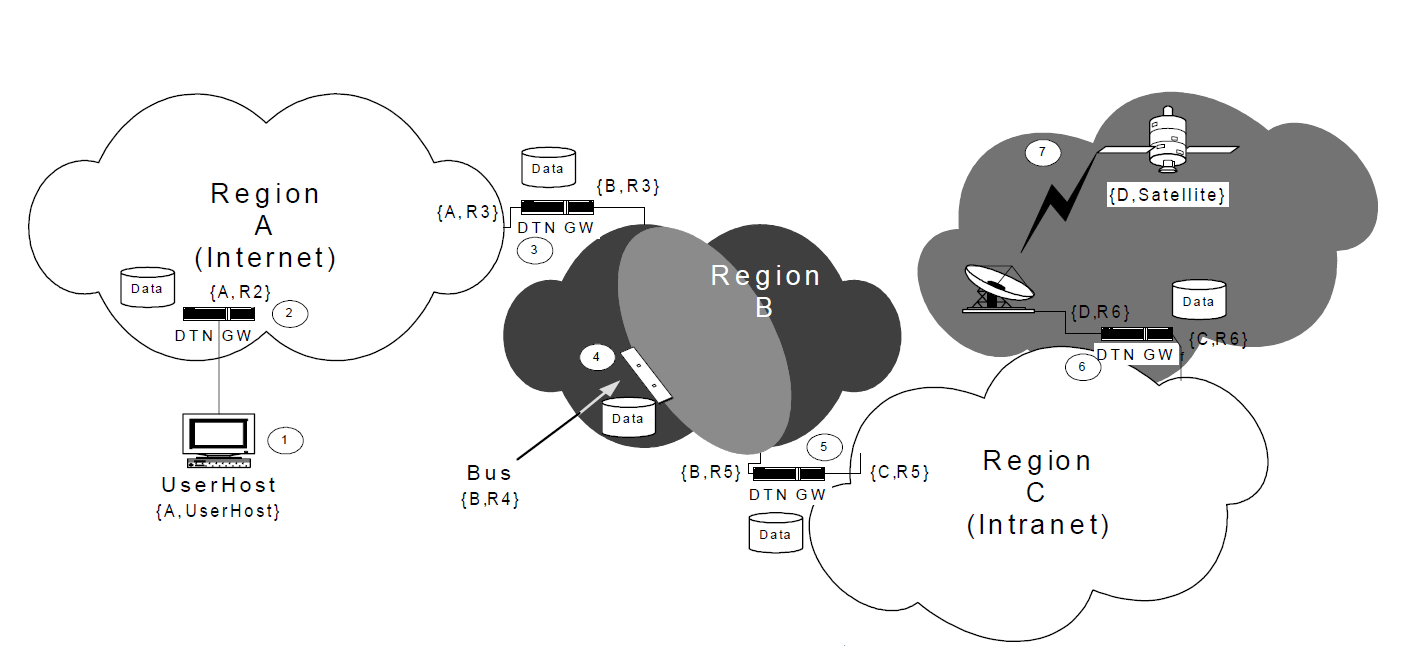
\includegraphics[width=\textwidth,natwidth=1420,natheight=672]{figures/dtn.png}
\caption{Overview of a Delay-Tolerant Network, cited from \cite{Kevin}}
\label{fig:dtn}
\end{figure}

It separates different challenged networks into ``regions" - within each region, nodes communicate under a same protocol, while different regions may run different protocols. As shown in the figure, region A uses Internet, region B uses a bus to deliver messages, region C uses its own Intranet and region C uses satellite to communicate. Different regions are connection by DTN gateways where messages from one region will be routed and forwarded to another region.

One of the key concept of DTN is custody transferring, which refers to the delivery of message from one DTN hop to another together with its reliable delivery responsibility - it's very much like delivering packages through a postal service. And using message couriers to achieve such custody transfer has been accepted as one practical implementation to overcome the difficulties in DTN \cite{Jain}\cite{Zhao}. Although the security issues of DTN have been discussed and evaluated in the high level design of the architecture \cite{Cerf}\cite{Scottrfc} (mainly to maintain efficient routing and prevent abuse of DTN), many security concerns still remain to be considered in the specific courier-dependent message delivery scenario (like what if the courier could be hijacked and examined?). Referencing the high level security framework pre-defined in the architecture, this project will dive into the detail of courier-dependent message delivery and create a practical and efficient security protocol for such scenario.

\subsection{Deniable Authentication}
Privacy protection has been taken much attention to since the communication through digital networks grows dramatically. Most network protocols require authentication as one of its essential steps to achieve secure communication. However, common authentications do not take privacy as one of its goals, thus they require revealing unique identifier of an entity to prove its identity to others - such like a digital signature or a piece of plaintext whose ciphertext can only be decrypted by the entity. As a matter of fact, it is this authentication mechanism disclose the identity of authenticator to third parties. Conversely, in many cases entities want to authenticate themselves to the target entities without revealing their identities to any third parties. This issues have been investigated and analysed by Abadi, who consequently introduced ``private authentication" and presented protocols meet the requirements \cite{Abadi}.

The concept of deniable authentication is created even earlier, by Dwork and Sahai \cite{Dwork}. It indicates the situation that an entity wishes to authenticate a message to the target entity while no any other entities can verify the authentication. Namely, the target entity can not prove the authenticity of the origin of the message to any other entities even itself is convinced by the authentication, thus the message creator can fully deny the existence of the message. It is extremely powerful in terms of privacy protection as combining with privacy authentication, no any private information will be leaked during the authentication. And its repudiation property is proved useful in applications like voting systems and commercial negotiation systems.

So far, many deniable authentication protocols have been invented, they can be sorted as two main classes - interactive \cite{Borisov} and non-interactive \cite{Xin}\cite{Wang}\cite{Shao}. Interactive deniable authentication requires at least 2 messages exchanged during the protocol, one forward and one reply. While non-interactive deniable authentication can achieve the goal in just one message with the cost of heavier computation.

This feature is added in the CDSP to provide an extra level of security to the message being exchanged in order to against potential malicious operations of couriers and message recipients. It might be very important in circumstances like military network or secret message delivery missions.

\section{Motivation and Objectives}
As stated above, this project is inspired by the notion of Delay-Tolerant Network and is specifically designated to create a protocol to improve the security and efficiency for one kind of its custody transferring - courier-dependent communication. More concretely, the invented CDSP should optimize courier-dependent communication in following aspects:
\begin{itemize}
\item Authentication \\
As the cost of such communication will be high - the transportation of courier could be costly, it requires any message delivery request must be authenticated by authorized entity and other entities should be able to check the validity of it.

\item Authenticity of Origin \\
The authenticity of origin of messages should be preserved during the communication, which means when message recipient gets the message, he is able to ensure the message creator. Meanwhile, it implies the integrity of message should be preserved.

\item Confidentiality of Message Content \\
The message content carried by courier should be kept confidential to any entities except the message creator and recipient. Because there is possibility that the courier could be compromised and data it carries may be examined by third parties, courier should gain no knowledge of the actual content it carries.

\item Efficiency \\
Due to the potential limitation of computing and storage capability of Courier and the high cost of such communication, protocol should be designed in such a way that it uses least number of messages and smallest message size to achieve the goal. Especially for cryptography operations, where overhead for encrypting/decrypting messages could be high.

\item Deniability \\
As mentioned above, in secret delivery missions, it would be plausible if Alice is able to deny sending the message in such a way that those who got the message can not prove its authentication to any third parties.
\end{itemize}

\noindent
At the end of the project, following objectives must be achieved:
\begin{enumerate}
\item A fully specified Courier-Dependent Security Protocol should be created and it should meet the requirements mentioned in the above list.
\item A Java library should be developed providing essential functions for implementing the protocol.
\item An application should be built to actually run this protocol.
\item A test of the application should be done to evaluate the performance of the protocol application.
\end{enumerate}

\section{Dissertation Structure}
In the rest of the dissertation, the detailed work will be presented. In Chapter 2 some related works will be discussed, and the differences of this project with those works will be highlighted. Then Chapter 3 will thoroughly describe the system that the protocol serves, including all set-ups, assumptions and rules. It is designated to convey a detailed picture of the scenario. Chapter 4 will fully illustrate the specification of CDSP with the help of message sequencing charts and afterwards, in Chapter 5, the security properties of it will be highlighted and verified. After that, the implementation of the protocol application will be demonstrated in Chapter 6. No concrete code but graphs and charts will be given to give a high level understanding of the work. Then it moves to Chapter 7, where the design of tests and evaluations of the application will be shown and some data will be analysed to show the performance of the protocol. Finally, Chapter 8 will summarise the achievements of the project and draw some reasonable conclusions by pointing out the current system limitation and potential improvements in future work.
\chapter{Background and Related Work}
\section{Background}
This project is not merged out of the void and the courier-dependent communication scenario is also not invented groundlessly. Some of the notions in this project have been introduced and discussed antecedently. To convey an entire overview of why this project is introduced and how it is designed, some details of the background information are given in this section.

\subsection{Delay-Tolerant Networks (DTN)}
Comparing to Internet which is relatively stable and reliable, so called ``challenged networks" are characterized by latency, bandwidth limitations, error probability, node longevity, or path stability that are substantially worse than is typical of today’s Internet \cite{Kevin}. The reason for causing the networks ``challenged" could be various - from geographical distances, lacking infrastructure to extreme environment conditions. Examples of such networks have been given by Fall, such as exotic media network - like near-earth satellite communication, and military ad-hoc networks. In order to achieve successful communication within such networks, instead of using TCP/IP - which will behave disappointingly \cite{Scott}, each challenged network may introduce its own protocol suits and network architectures to meet their specific needs. However, the diversity of these various protocols and architectures prevents those networks to communicate with each other and it has been justified by Fall \cite{Kevin} that simple link-repair approaches is not sufficient to solve the whole problem.

Then the architecture of Delay-Tolerant Network (DTN) was introduced to tackle the problem. Basically it achieve communication between various disparate challenged networks with significantly different sets of physical and operational constraints (latency, stability, etc.) by adding another layer of protocol to the local protocol stack. The Figure \ref{fig:dtn} briefly illustrates the architecture of a delay-tolerant network.

\begin{figure}[h!]
\centering
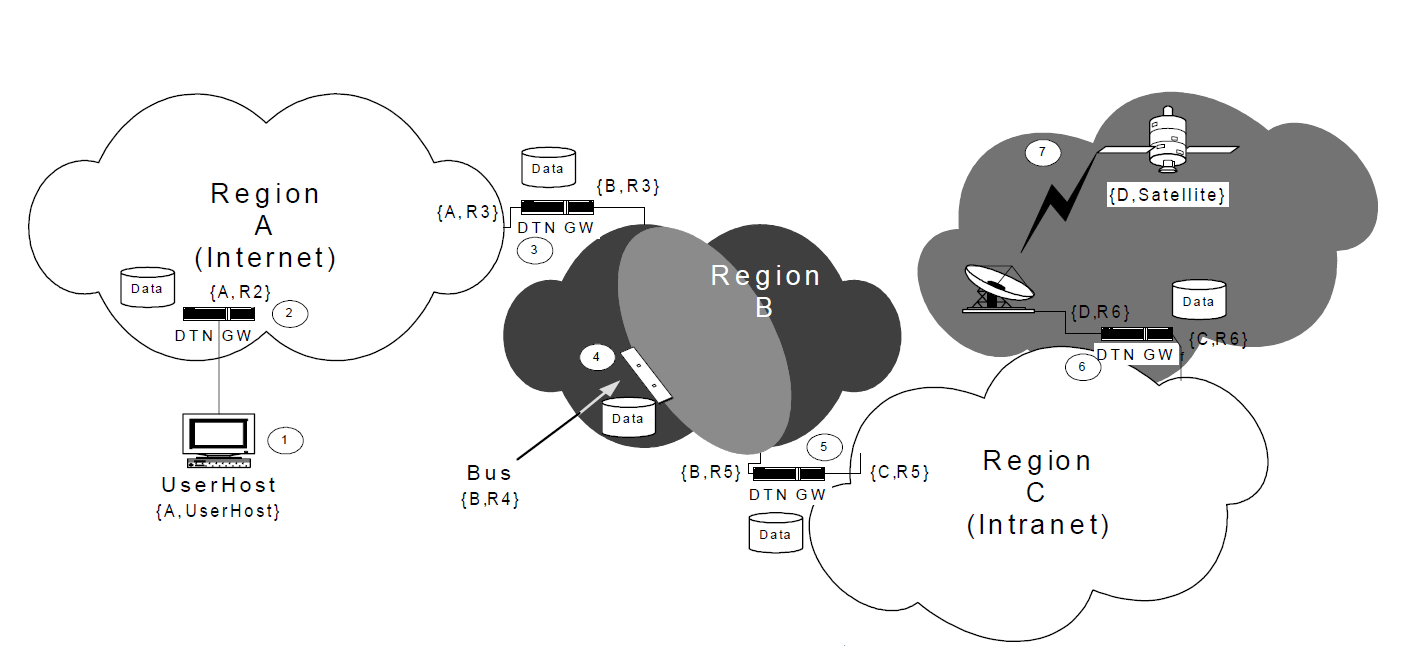
\includegraphics[width=\textwidth,natwidth=1420,natheight=672]{figures/dtn.png}
\caption{Overview of a Delay-Tolerant Network, cited from \cite{Kevin}}
\label{fig:dtn}
\end{figure}

It separates different challenged networks into ``regions" - within each region, nodes communicate under a same protocol, while different regions may run different protocols. As shown in the figure, region A uses Internet, region B uses a bus to deliver messages, region C uses its own Intranet and region C uses satellite to communicate. Different regions are connection by DTN gateways where messages from one region will be routed and forwarded to another region.

One of the key concept of DTN is custody transfer, which refers to the delivery of message from one DTN hop to another together with its reliable delivery responsibility - it's very much like delivering packages through a postal service. And using message couriers to achieve such custody transfer has been accepted as one practical implementation to overcome the difficulties in DTN \cite{Jain}\cite{Zhao}. The scenario introduced in this project is a concrete instance of such custody transfer and the network our CDSP works in is also referred to an instance of challenged network.

Although the security issues of DTN have been discussed and evaluated in the high level design of the architecture \cite{Cerf}\cite{Scottrfc}, such like essential authentication and message integrity preservation, etc., they are specially designed to maintain efficient routing and prevent abuse of DTN, many other security concerns still remain to be considered in the specific courier-dependent message delivery scenario (like what if the courier could be hijacked and examined?). Referencing the high level security framework pre-defined in the architecture, this project will dive into the detail of courier-dependent message delivery and create a practical and efficient security protocol for the specific scenario.

\subsection{Deniable Authentication}
Privacy protection has been taken much attention to since the communication through digital networks grows dramatically. Most network protocols require authentication as one of its essential steps to achieve secure communication. However, common authentication methods do not take privacy as one of its goals, thus they require explicitly showing entity's unique identifier to prove its identity to others - such like a digital signature or a piece of plaintext whose ciphertext can only be decrypted by the entity. As a matter of fact, it is this authentication mechanism disclose the identity of authenticator to third parties as the identifier is exposed to any eavesdropper. Conversely, in many cases entities want to authenticate themselves to the target entities without revealing their identities to any third parties. This issues have been investigated and analysed by Abadi, who consequently introduced ``private authentication" and presented protocols meet the requirements \cite{Abadi}.

The concept of deniable authentication is created even earlier, by Dwork and Sahai \cite{Dwork}. Different with private authentication, it indicates the situation that an entity wishes to authenticate a message to the target entity while no any other entities can verify the authentication. Namely, the target entity can not prove the authenticity of the origin of the message to any other entities even itself is convinced by the authentication, thus the message creator can fully deny creating the message at all. It is extremely powerful in terms of privacy protection - combining with privacy authentication, no any private information will be leaked during the authentication. And its repudiation property is proved useful in applications like voting systems and commercial negotiation systems.

So far, many deniable authentication protocols have been invented, they can be sorted as two main classes - interactive \cite{Borisov} and non-interactive \cite{Xin}\cite{Wang}\cite{Shao}. Interactive deniable authentication involves interaction between entities, it requires at least 2 messages exchanged during the protocol, one forward and one reply. While non-interactive deniable authentication can achieve the goal in just one forward message with the cost of heavier computation.

This feature is added in the CDSP to provide an extra level of security to the message being exchanged in order to against potential malicious operations of couriers and message recipients. It might be very important in circumstances like military network or secret message delivery missions.

\section{Related Work}
Since the Delay-Tolerant Network architecture is first introduced, its security concerns have drawn the attention of relative research groups. Soon, much effort has been put on analysing the practicality of security implementation in DTNs and many designs have been made. Here two of security protocols which considered similar to this project are introduced as references.

\subsection{Bundle Security Protocol \cite{Symington}}
Soon after the release of DTN architecture specification \cite{Cerf}, a protocol called Bundle Protocol \cite{Scottrfc} is designed and documented by Scott et al., which formally defines the format of messages (named bundles) exchanged between each end-to-end entities and abstracts the services provided by DTNs. Analogous to TCP/IP providing end-to-end connectivity specifying how data is formatted, addressed, transmitted, routed and received between originator and destination in Internet, Bundle Protocol takes care of those issues for every DTN hops. Figure~\ref{fig:bundleblockformat} shows the the basic block formats in bundle protocol. Basically, it defines that a single bundle should contain one primary bundle block and arbitrary number of bundle payload blocks. The primary bundle block is strictly formatted, it describes the information about the whole bundle,  while each bundle payload block provides different services that can be totally independent to each other and its format is relatively free to extend. This message structure is designed for extension as new functions could be easily added to the protocol by defining another new type of bundle payload block.

\begin{figure}[h!]
\centering
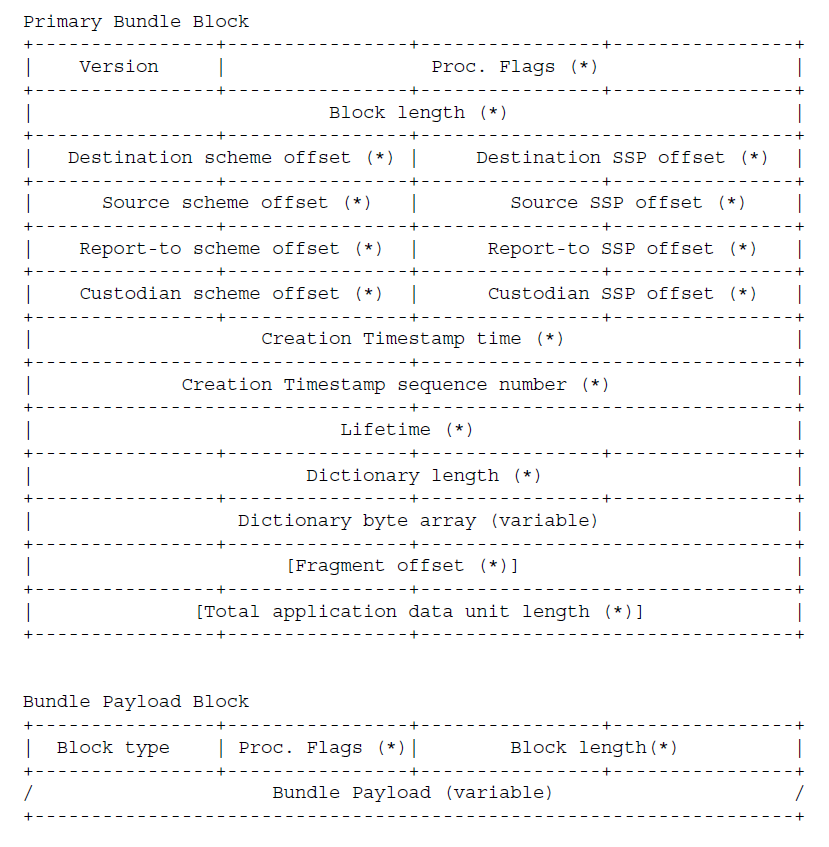
\includegraphics[width=\textwidth,natwidth=829,natheight=847]{figures/bundleblockformat.png}
\caption{Message Format of Bundle Protocol \cite{Scottrfc}}
\label{fig:bundleblockformat}
\end{figure}

The Bundle Security Protocol is one of extensions of Bundle Protocol. It is designated to provide data integrity and confidentiality protection for the Bundle Protocol. The main contribution is defining 4 new types of bundle payload block - BundleAuthenticationBlock, PayloadIntegrityBlock, PayloadConfidentialityBlock and ExtensionSecurityBlock. Those new types of blocks - as their name stated, can be appended to any bundle to add an extra level of corresponding security protection to it. For example, if a bundle needs to be authenticated, the originator should add an extra bundle payload block to the original bundle, formatted as a BundleAuthenticationBlock. Thus the authentication of the bundle can be checked in every DTN hop during the transmission.

Bundle Security Protocol has defined the security issues of DTNs in a high level, it ensures the secure message transmission between originator and receiver connected by hops. However, the detailed operations between hop to hop is not covered by this protocol. Referring to the architecture of DTN, every end-to-end nodes are linked by hops, and the message transmission from one hop to the next is called custody transfer. The implementation of custody transfer can be various, but a common method is courier-dependent transferring. In Bundle Security Protocol, such custody transfer is assumed to be accomplished securely and efficiently so that it only cares about the higher level. Unfortunately, it is not always the case. Every custody transfer can be complicated and extra work should be done to keep it functioning. Thus this project will explore the specific scenario of courier-dependent custody transfer and create a protocol for it. Although the message format of Bundle Security Protocol is highly referential, it still not quite fit the scenario we discussed before. The major problem is: as a general protocol it has a very heavy overhead to maintain the consistency of different blocks and extensions, which seems redundant in our scenario. So comparing to the Bundle Security Protocol, the newly created protocol will use less-sized messages and be more problem specific.

\subsection{DTN Anonymity and Secure Architecture \cite{Kate}}
The DTN Anonymity and Secure Architecture (DASA) is inspired by Seth et al. who tried to find a secure solution for helping rural areas to get continuous Internet access despite its long-period disconnection \cite{Seth}\cite{SethKeshav}. Although specific situations could be various in rural areas, Seth et al.'s study comes up with an unified approach: buses with wifi-based access and storage capability periodically drive past each villages and collect data from users in villages. Then buses carry the data to the nearest local Internet gateway and send out the data collected. Figure~\ref{fig:ruralarea} roughly illustrates the scenario. Basically, Seth et al.'s architecture achieves the secure communication between each user and buses in such a way that every data delivery from user to bus must be mutually authenticated. Based on this achievement, Kate et al. abstracts the scenario such that it not only applies to rural area networks but also any generic DTNs. Furthermore, Kate et al. also adds two more security properties to the original architecture - data confidentiality and anonymity, forming the DTN Anonymity and Secure Architecture.

\begin{figure}[h!]
\centering
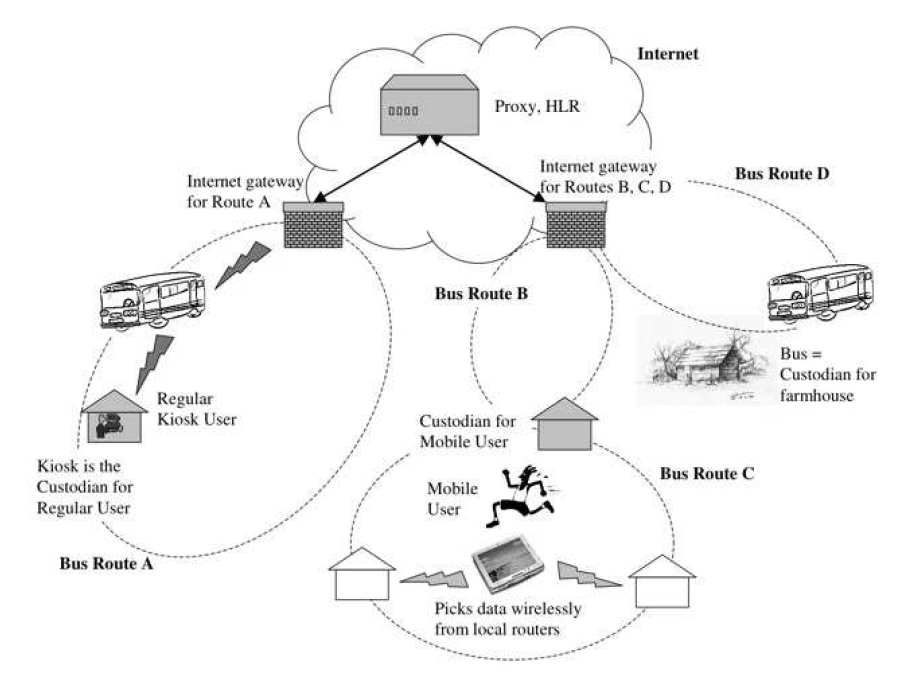
\includegraphics[width=\textwidth,natwidth=913,natheight=682]{figures/ruralarea.png}
\caption{Rural Area DTN \cite{Seth}}
\label{fig:ruralarea}
\end{figure}

The DTN Anonymity and Secure Architecture is very close to the scenario of this project - buses can be regarded as couriers who carry the message for end users, and the protocol used in this architecture takes care of the authentication processes between end users and the buses, and it also conceals the identity of end users. However, there are still some points remain controversial: (1) It does not hide the message content from the DTN router (courier), so the message content will be totally exposed once the DTN router is compromised. (2) It requires mutual authentication when end node transmit message to a DTN router (courier). Normally, mutual authentication either is interactive or demands extra assumptions - such as in Sakai-Ohgishi-Kasahara (SOK) Key Agreement Scheme \cite{Sakai}, it needs a trusted third party ``private key generator", which increases the system complexity, thus one way authentication might be a better choice. (3) Its anonymity mechanism highly relies on the trusted third party ``private key generator" which may or may not be introduced in the system. (4) The message sent from end users is not fully deniable. According to the specification of its anonymity mechanism, it only conceals the sender identity behind a group of valid users identities. Although the courier does not know the true identity of sender, it at least can prove that one of the member in the group created the message to a third party.

In summary, the DTN Anonymity and Secure Architecture sets up a scenario similar to our project's courier-dependent scenario, and some methods it uses to achieve security protection is inspiring. However above 4 points show that in order to fully fit the scenario of this project, some improvements still need to be done.
\chapter{System Description}
\section{System Model}
\subsection{Overview}
This protocol is typically used under the scenario that there is no reliable or stable networks existed between communication entities (called Alice and Bob). Entities under such conditions can be abstracted as off-line entities in the sense that their network is restricted and can not reach the others' networks. This system allows those off-line entities to communicate by using a Courier to deliver the message. Assuming Alice wants to send a message to Bob, the Courier firstly gets the message from Alice and stores it, then physically transport to Bob and send the message to Bob. \par
The goal of this protocol is to ensure the message from Alice to Bob is secure in the sense that no one can reveal its content but Bob. To achieve that, the Courier should never be trusted, which means the real content of the message should not be accessed by Courier and both Alice and Bob are able to deny the communication with Courier at any time. Furthermore, to prevent sensitive information from being leaked by malicious message recipient (Bob), message creator (Alice) should be able to deny the message content as well.

\subsection{Initial Set-ups}
According to the description above, totally 3 different types of entities are defined in the protocol - Alice, Bob and Courier. Following specification lists the notations and jobs of all 3 entities together with the information they should hold before running the protocol:

\begin{itemize}
\item Alice $\mathcal{A}$ denotes a set of devices who create the message and waits it to be delivered, so it is also called ``message creator". It possesses an unique $\mathcal{ID} \in \{0, 1\}^*$, a secret key $sk_A$ as part of its asymmetric key pair, and the message $\mathcal{M}$ to be sent. \\
$\mathcal{A}$'s ID and public key should be known by at least one Courier so that it will be connected by Courier.

\item Bob $\mathcal{B}$ denotes a set of devices who wait incoming messages delivered by Courier, so it is also called ``message recipient". It possesses an unique $\mathcal{ID} \in \{0, 1\}^*$, and a secret key $sk_B$ as part of its asymmetric key pair.\\
Similarly, its ID and public key should also be known by at least one Courier.

\item Courier $\mathcal{C}$ denotes a set of devices who carry the message of Alice, physically transport from Alice to Bob, and deliver the message to Bob. Initially it only possesses an unique $\mathcal{ID} \in \{0, 1\}^*$ and at least a contact $\mathcal{ID} \in \{0, 1\}^*$ and its corresponding public key, specifies the entity it is going to contact.\\
However, a single Courier will play two different roles in the protocol run - one receives message from Alice, one delivers message to Bob. They are denoted as $\mathcal{CR}$ (Courier Receiver) and $\mathcal{CS}$ (Courier Sender) in the protocol specification. In addition to $\mathcal{CR}$, $\mathcal{CS}$ possesses some more information: the $\mathcal{ID}$ of the message creator and the encrypted message received from $\mathcal{A}$.
\end{itemize}

\paragraph{Public Key Distribution}
The distribution of asymmetric key pairs used for authentication is out of the scope of this protocol, thus $\mathcal{A}$ and $\mathcal{B}$ are assumed to hold their asymmetric key pairs before running the protocol. Furthermore, all entities in the system are assumed to know each other's public key (does not matter it is distributed with manufacture, authenticated by CA, or by key exchange), before running the protocol.

\paragraph{Devices v.s. Entities}
A device $x$ denotes a physical object that runs the protocol. Differently, an entity denotes a particular role in the running of the protocol. It should be noted that any  device can run multiple instances of this protocol with other devices simultaneously, thus a single device can be any three entities at the same time. The role it plays in different communications is defined by what information $x$ holds and what sub-protocol it runs (will be described in Communication Model). However, an entity in the protocol can be associated with only one device.

\subsection{Communication Model}
Ultimately, every single run of this protocol achieves an abstract M-to-1 communication - a certain number of devices $a_0, a_1, ... a_M \in \mathcal{A}$ send message to a single device $b \in \mathcal{B}$ independently, using a device $c \in \mathcal{C}$ as media. As physical transportation is extremely slow and costly compare to network communication, the total number of physical transportation should be reduced to minimum. The optimized solution appeared to be separating the protocol into two main phases - Message Acquisition phase and Message Delivery phase. Assume off-line devices $a_1, a_2, ... a_M \in \mathcal{A}$ need to send message to the off-line device $b \in \mathcal{B}$. In Message Acquisition phase, a Courier will physically transport to every $a \in \mathcal{A}$, connect to it and get the message that is for the $b$. After the Courier collects all needed messages, it enters Message Delivery phase, where the Courier transports to $b$ and transmit all acquired messages to it.

According to explanation above, the whole task can be divided into M + 1 individual communications. Every such individual communication happens between a Courier $c \in \mathcal{C}$ and one of $\mathcal{A} \cup \mathcal{B}$ after the Courier connects to the target. All these communications use one of typical network communication methods (e.g. cable, Wifi, Bluetooth, etc.) and apply its corresponding communication protocols (e.g. TCP/IP, UDP, Bluetooth protocol, etc.). The following figure shows how the communication is organized.

\begin{figure}[h!]
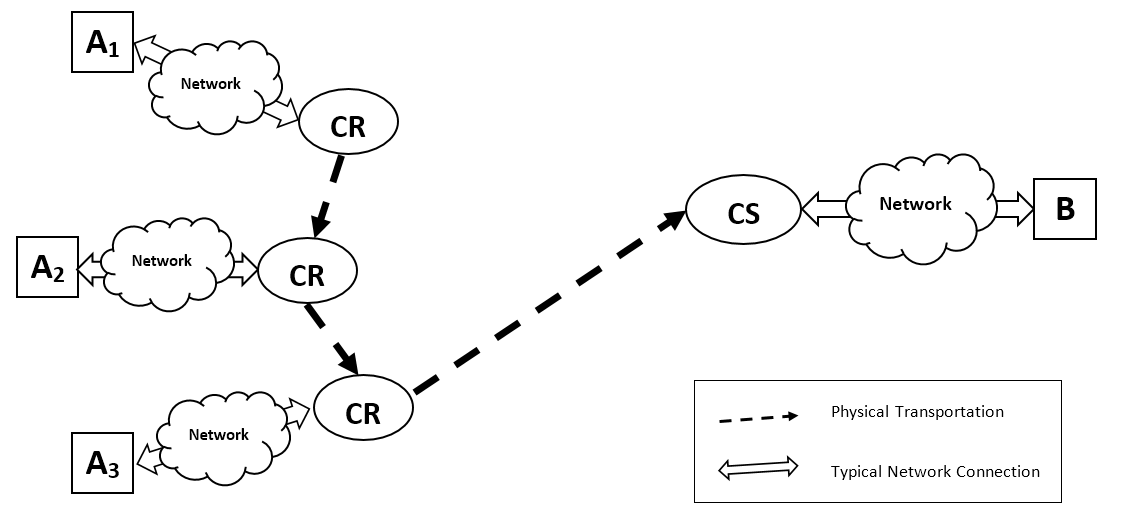
\includegraphics[width=\textwidth,natwidth=1123,natheight=530]{figures/communicationmodel.png}
\caption{Communication Model}
\end{figure}

The figure "Communication Model" illustrates the procedure of a 3-to-1 communication. The Courier first connects to A$_1$, be the role of $\mathcal{CR}$, and gets A$_1$'s message for B through the connection, then disconnects and transports to A$_2$. It should do the same thing to A$_2$ and then transport to A$_3$. After it collects all data from A$_1$, A$_2$ and A$_3$, it transports to B and be the role of $\mathcal{CS}$ to send all collected messages to B. The networks between Courier and As or B can be any kind of connection and do not to be the same, as long as both entities accept. 

To define different kinds of communication, this protocol consists of 2 sub-protocols - a) Submit protocol: how message is submitted from $\mathcal{A}$ to $\mathcal{C}$; b) Transmit protocol: after $\mathcal{C}$ gets connected with $\mathcal{B}$, how message is transmitted to $\mathcal{B}$. These two sub-protocols ensure the secure transmission of message from $\mathcal{A}$ to $\mathcal{B}$ and they will be analysed in the later part.

\subsection{Honest Entity Behaviour}
Generally, all 3 entities in this protocol act as devices who possess their own initial information (described above), take $\mathcal{M}$ as input, and output $\mathcal{M'}$. All honest entities in this protocol should follow the following procedure:
\begin{enumerate}
\item If entity is $\mathcal{C}$, initiate the protocol by sending ${\mathcal{M}_0}'$, otherwise ignore this step.
\item Wait for $\mathcal{M}_1$
\item Receive $\mathcal{M}_1$, decrypt all its ciphertexts and reveal their contents if applicable.
\item Check validity of the contents of $\mathcal{M}_1$ (e.g. check message format, check sender ID, receiver ID, digital signature or MAC, if applicable). If any check violates, immediately report ``Protocol Error" and abort the session.
\item Process the message content (e.g. print the result, stores the contents in local storage).
\item Prepare and send message ${\mathcal{M}_1}'$. If no message to send, abort the session silently.
\item Back to step 2.
\end{enumerate}

However, three entities have different behaviour patterns, they will be specified here, respectively:
\paragraph{Alice $\mathcal{A}$}
\begin{itemize}
\item An entity $a \in \mathcal{A}$ create the message to send, and prepare its meta data. Then it continuously listening to its network, waiting for incoming Couriers.

\item Alice will submit its message to any Courier who request for it. When submitting, the message recipient must be explicitly specified.

\item Alice is allowed to submit any message arbitrary times, to single or multiple Couriers. Alice itself should not care who carries the message, nor how many Couriers carry the message.

\item During an uncompleted session, if no response from Courier for a long time, Alice should be able to detect the timeout, cancel the effects of previous actions in this session and abort the session voluntarily.

\item If the message is not successfully sent, Alice should wait for next Couriers to send this message.
\end{itemize}

\paragraph{Bob $\mathcal{B}$}
\begin{itemize}
\item An entity $b \in \mathcal{B}$ must be continuously listening to its network, waiting for incoming messages.

\item Bob will download all messages from any Courier who transmits. If any message from $\mathcal{A}$ is invalid, Bob simply discards it.

\item Bob will discard all duplicated messages. Duplicated message are defined as messages whose Meta Signature are exactly the same. Because message Meta contains its creator ID and timestamp, same Meta reflects those messages are created by the same entity at the exact same time.

\item During an uncompleted session, if no response from Courier for a long time, Bob should be able to detect the timeout, cancel the effects of previous actions in this session and abort the session voluntarily.
\end{itemize}

\paragraph{Courier $\mathcal{C}$}
\begin{itemize}
\item As Courier's physical transportation is a very complicated task, it is out of the scope of this protocol. It is assumed that Courier is carried by an intelligent agent (such like human) who always knows where the Courier should transport to.

\item Courier should transport to every $a \in \mathcal{A}$ one by one and get their messages if there are any. Courier should be capable of storing those data for a long time.

\item After collect messages from all $a$ in the list, Courier should transport to every $b$ that is the recipient of the Courier and deliver all messages to them. If the receipt from $b$ violates the messages Courier just sent, Courier should resend the messages by restart the session again.

\item Once a full protocol run has been completed, all relative data stored in Courier is expired and should not affect future run of protocol.
\end{itemize}

\section{Adversary Model}
The adversary model in this protocol is mostly derived from Dolev-Yao model which implies ``adversary carries the message" \cite{Dolev}. Moreover, the adversary can also do something special in this protocol system. Specifically, adversary $\mathcal{Z}$ has following capabilities:
\begin{itemize}
\item It supervises the whole network system, which means it knows when, where and how any two entities are communicating, and it knows which entity possesses what information.
\item It can access/rewrite any message passing through the network.
\item It is a legitimate user of the network and it can be any of 3 entities in this protocol.
\item It can access to all the Courier's data at any stage of the protocol.
\item Any $a \in \mathcal{A}$ or $b \in \mathcal{B}$ will always have the opportunity to be connected by any $c \in \mathcal{C}$, which means an adversary will always have opportunity to be contacted by any honest entities.
\end{itemize}

It should be noted that this protocol, same as all other network protocols, is vulnerable to DoS attacks. $\mathcal{Z}$ can always prevent a message from being sent, thus it will not be covered in the security analysis.
\section*{Protocol Specification}
A successful run of CDSProtocol consists of 3 stages - (1) message creators submit their messages to a single courier. (2) courier physically transports to the message receiver. (3) courier transmits the messages to the message receiver. As controlling couriers and  planning couriers' routes are out of the scope of this protocol, it is assumed that in this protocol, couriers eventually are able to approach the target. Therefore stage (2) will not be discussed here. \par
The protocol specification will focus on the other two stages - (1) and (3), we call them Message Acquisition phase and Message Delivery phase. To ensure secure communication in both two phases, two sub-protocols - Submit Protocol and Transmit Protocol, are defined for two phases respectively. The Submit Protocol runs between Alice and Courier, while the Transmit Protocol runs between Bob and Courier. As those two sub-protocols can be run independently, they will be explained separately.
\subsection{Notations}
\paragraph{Concatenation \textbar\textbar :}
It denotes the operation that concatenates two pieces of data together. For example ``A\textbar\textbar B" simply means appending B to A.
\paragraph{Repeat concatenation $^+$ :}
It represents a piece of data concatenates itself one or many times. For example ``A$^+$" equals a sequence of A concatenated together, which can be ``A" or ``A\textbar\textbar A" or ``A\textbar\textbar A\textbar\textbar  ..." where A occurs at least once.
\subsection{Submit Protocol}
\subsubsection{Preconditions}
\begin{itemize}
\item Alice holds a unique pair of asymmetric key ($pk_A$, $sk_A$)
\item Courier knows Alice's public key $pk_A$
\end{itemize}
\subsubsection{Postconditions}
\begin{itemize}
\item Alice knows all the messages have been successfully sent to someone
\item Alice doesn't know the identity of the receiver
\item Alice doesn't know whether the message will be eventually deliver to Bob
\item Courier knows the integrity of the message is preserved
\item Courier knows the authenticity of origin of Alice's messages
\end{itemize}

\subsubsection{Message Sequencing Chart}
\begin{msc}{Submit Protocol}
\setlength{\instdist}{3\instdist}
\setlength{\envinstdist}{2\envinstdist}
\setlength{\levelheight}{1.5\levelheight}
\declinst{alice}{Alice}{}
\declinst{courier}{Courier}{}

\action*{pick a random key k$_C$}{courier}
\nextlevel[2]
\mess{1: Courier\textbar\textbar size\textbar\textbar E$_{pk_A}$(k$_C$)}{courier}{alice}
\nextlevel
\action*{pick symmetric key k$_{AB}$}{alice}
\nextlevel
\action*{Meta = E$_{pk_B}$(k$_{AB}$\textbar\textbar Alice\textbar\textbar Bob\textbar\textbar timestamp)}{alice}
\nextlevel
\action*{MetaS = E$_{k_{AB}}$(SIGN$_A$(Meta))}{alice}
\nextlevel
\action*{Msg = E$_{k_{AB}}$(message content)}{alice}
\nextlevel
\action*{MsgM = MAC$_{k_{AB}}$(Msg)}{alice}
\nextlevel
\action*{Infos = Alice\textbar\textbar Bob\textbar\textbar Meta\textbar\textbar MetaS\textbar\textbar Msg\textbar\textbar MsgM}{alice}
\nextlevel[2]
\mess{2: Infos\textbar\textbar MAC$_{k_C}$(Infos)}{alice}{courier}
\nextlevel
\action*{check validity of MAC$_{k_C}$(Infos)}{courier}
\nextlevel
\action*{check validity of sender ID}{courier}
\nextlevel
\action*{check size of Infos}{courier}
\nextlevel[2]
\mess{3: MAC$_{k_C}$(message 2)}{courier}{alice}
\nextlevel
\action*{check validity of MAC$_{k_C}$(message 2)}{alice}
\nextlevel
\end{msc}
\\


\subsubsection{Specification}
\begin{enumerate}
\item Courier randomly creates a symmetric key $k_C$. The key will be sent to Alice and used for deniable authentication.

\item Courier connects to Alice and sends message 1 to Alice. Message 1 should contain (1) The $\mathcal{ID}$ of Courier, (2) The maximum storage size of Courier, (3) Random key $k_C$ encrypted by Alice's public key.

\item Alice randomly creates a symmetric key $ k_{AB} $. The key is supposed to be the session key with Bob.

\item Alice prepares the Meta block, which is an encrypted block under the public key of Bob. The plaintext of Meta contains (1) Symmetric key $ k_{AB} $, (2) The $ \mathcal{ID} $ of Alice, (3) The $ \mathcal{ID} $ of Bob, (4) A timestamp indicates the time Alice creates this message.

\item Alice creates a MetaS block which is an encrypted digital signature of Meta, under the key $ k_{AB} $.

\item Alice creates the Msg block. Alice encrypts the message for Bob under $ k_{AB} $.

\item Alice creates a MsgM block, which is the MAC of Msg, created under the $ k_{AB} $.

\item Alice creates a Infos block, which is the concatenation of (1) The $ \mathcal{ID} $ of Alice, (2) The $ \mathcal{ID} $ of Bob, (3) Meta block, (4) MetaS block, (5) Msg block, (6) MsgM block.

\item Alice prepares message 2. Alice first reveals $ k_C $ by decrypting E$_{pk_A}$(k$_C$) in message 1, using $ sk_A $. Then it creates a MAC of the Infos block under $ k_C $ and appends the $ \mathcal{MAC}_{k_C} $ to the Infos block, forming message 2.

\item Alice examines the size of Infos block and sends out message 2. If the total size of Meta, MetaS, Msg, MsgM blocks exceeds the storage limitation of Courier, it either reduces the size of those blocks and prepares them again, or reports an error and aborts the protocol. If it doesn't, Alice sends the whole message 2 to Courier.

\item Courier checks the validity of message 2. It first verifies $ \mathcal{MAC}_{k_C} $(Infos), if true, then checks the $ \mathcal{ID} $ of Alice. After that, it checks the total size of the Meta, MetaS, Msg and MsgM blocks, making sure it does not exceeds the storage limitation. If any of above checks violate, Courier should report an error and abort the protocol.

\item Courier prepares message 3. Courier uses $ k_C $ to create a MAC of whole message 2 which is received from Alice. 

\item Alice checks the validation of message 3. Alice verifies the received MAC using $ k_C $. If it verifies false, Alice knows its message may not be successfully sent, it means the protocol fails. Otherwise, the protocol successes.
\end{enumerate}

\pagebreak
\subsection{Transmit Protocol}
\subsubsection{Preconditions}
\begin{itemize}
\item Bob holds a unique pair of asymmetric key ($pk_B$, $sk_B$)
\item Courier knows Bob's public key $pk_B$
\end{itemize}
\subsubsection{Postconditions}
\begin{itemize}
\item Bob accepts the message, knowing it is created by Alice
\item Bob doesn't know the identity of the message sender
\item Courier knows Bob has successfully received and accepted the message
\end{itemize}
\subsubsection{Message Sequencing Chart}
\begin{msc}{Transmit Protocol}
\setlength{\instdist}{3\instdist}
\setlength{\envinstdist}{2\envinstdist}
\setlength{\levelheight}{1.5\levelheight}
\declinst{bob}{Bob}{}
\declinst{courier}{Courier}{}

\action*{pick a random key k$_C$}{courier}
\nextlevel
\action*{concatenate all Data blocks for Bob}{courier}
\nextlevel[2]
\mess{1: Courier\textbar\textbar E$_{pk_B}$(k$_C$)\textbar\textbar Data$^+$}{courier}{bob}
\nextlevel
\action*{check validity of all Data blocks}{bob}
\nextlevel[2]
\mess{2: MAC$_{k_C}$(message 1)}{bob}{courier}
\nextlevel
\action*{check validity of MAC$_{k_C}$(message 1)}{courier}
\nextlevel
\end{msc}
\\
where: \\
Data = Meta\textbar\textbar MetaS\textbar\textbar Msg\textbar\textbar MsgM\\
Meta = E$_{pk_B}$(k$_{AB}$\textbar\textbar Alice\textbar\textbar Bob\textbar\textbar timestamp)\\
MetaS = E$_{k_{AB}}$(SIGN$_A$(Meta))\\
Msg = E$_{k_{AB}}$(message content)\\
MsgM = MAC$_{k_{AB}}$(Msg)

\subsubsection{Specification}
\begin{enumerate}
\item Courier randomly creates a symmetric key $k_C$. The key will be sent to Bob and used for deniable authentication.

\item Courier prepares the data for Bob. Courier searches for all early collected Data blocks for Bob, each Data block is the concatenation of (1) Meta block, (2) MetaS block, (3) Msg block, (4) MsgM block. Courier then concatenates all founded Data blocks, forming Data$^+$ block.

\item Courier connects to Bob and sends message 1 to Bob. Message 1 contains (1) The $\mathcal{ID}$ of Courier, (2) Random key $ k_C $ encrypted by Bob's public key, (3) The concatenation of all Data blocks for Bob.

\item Bob receives message 1 and checks the validity of all Data blocks received. Specifically, for checking every Data block, it should do the following steps:
 \begin{enumerate}
 \item use $ sk_A $ to decrypt Meta, and reveal $ k_{AB} $, message creator's ID, message recipient ID and timestamp.
 \item check if message recipient ID is Bob itself and check timestamp to see if this message is expired.
 \item use $ k_{AB} $ to decrypt MetaS and reveal SIGN$_A$(Meta).
 \item verify SIGN$_A$(Meta) using $ pk_A $.
 \item verify MsgM using $ pk_A $.
 \item use $ pk_A $ to decrypt Msg and reveal the message content sent.
 \end{enumerate}
If any violation occurs during the checking or verification in certain Data block, Bob just discards the Data block and continues checking other blocks if any.

\item Bob prepares message 2. Bob first reveals $ k_C $ by decrypting E$_{pk_B}$(k$_C$) in message 1, using $ sk_B $. Then Bob uses $ k_C $ to create a MAC of whole message 1 which is received from Courier. 

\item Courier checks the validation of message 2. Courier verifies the received MAC using $ k_C $. If it verifies false, Courier knows its message may not be successfully sent, it means the protocol fails. Otherwise, the protocol successes.
\end{enumerate}

\section*{Security Analysis}
\subsection*{System Model}
\subsubsection*{Overview}
This protocol is typically used under the scenario that there is no reliable or stable networks existed between communication entities (called Alice and Bob). Entities under such conditions can be abstracted as off-line entities in the sense that their network is restricted and can not reach the others' networks. This system allows those off-line entities to communicate by using a Courier to deliver the message. Assuming Alice wants to send a message to Bob, the Courier firstly gets the message from Alice and stores it, then physically transport to Bob and send the message to Bob. \par
The goal of this protocol is to ensure the message from Alice to Bob is secure in the sense that no one can reveal its content but Bob. To achieve that, the Courier should never be trusted, which means the real content of the message should not be accessed by Courier and both Alice and Bob are able to deny the communication with Courier at any time. Furthermore, to prevent sensitive information from being leaked by malicious message recipient (Bob), message creator (Alice) should be able to deny the message content as well.

\subsubsection*{Initial Set-ups}
According to the description above, totally 3 different types of entities are defined in the protocol - Alice, Bob and Courier. Following specification lists the notations and jobs of all 3 entities together with the information they should hold before running the protocol:

\begin{itemize}
\item Alice $\mathcal{A}$ denotes a set of devices who create the message and waits it to be delivered. It possesses an unique $\mathcal{ID} \in \{0, 1\}^*$, a secret key $sk_A$ as part of its asymmetric key pair, and the message $\mathcal{M}$ to be sent. \\
$\mathcal{A}$'s ID and public key should be known by at least one Courier so that it will be connected by Courier.

\item Bob $\mathcal{B}$ denotes a set of devices who wait incoming messages delivered by Courier. It possesses an unique $\mathcal{ID} \in \{0, 1\}^*$, and a secret key $sk_B$ as part of its asymmetric key pair.\\
Similarly, its ID and public key should also be known by at least one Courier.

\item Courier $\mathcal{C}$ denotes a set of devices who carry the message of Alice, physically transport from Alice to Bob, and deliver the message to Bob. Initially it only possesses an unique $\mathcal{ID} \in \{0, 1\}^*$ and at least a contact $\mathcal{ID} \in \{0, 1\}^*$ and its corresponding public key, specifies the entity it is going to contact.\\
However, a single Courier will play two different roles in the protocol run - one receives message from Alice, one delivers message to Bob. They are denoted as $\mathcal{CR}$ (Courier Receiver) and $\mathcal{CS}$ (Courier Sender) in the protocol specification. In addition to $\mathcal{CR}$, $\mathcal{CS}$ possesses some more information: the $\mathcal{ID}$ of the message creator and the encrypted message $\mathcal{E(M)}$ received from $\mathcal{A}$.
\end{itemize}

\paragraph{Public Key Distribution}
The distribution of asymmetric key pairs used for authentication is out of the scope of this protocol, thus $\mathcal{A}$ and $\mathcal{B}$ are assumed to hold their asymmetric key pairs before running the protocol. Furthermore, all entities in the system are assumed to know each other's public key (does not matter it is distributed with manufacture, authenticated by CA, or by key exchange).

\paragraph{Devices v.s. Entities}
A device $x$ denotes a physical object that runs the protocol. Differently, an entity denotes a particular role in the running of the protocol. It should be noted that any  device can run multiple instances of this protocol with other devices simultaneously, thus a single device can be any three entities at the same time. The role it plays in different communications is defined by what information $x$ holds and what sub-protocol it runs (will be described in Communication Model). However, an entity in the protocol can be associated with only one device.

\subsubsection*{Communication Model}
Ultimately, every single run of this protocol achieves an abstract M-to-1 communication - a certain number of devices $a_0, a_1, ... a_M \in \mathcal{A}$ send message to a single device $b_0, b_1, ..., b_M \in \mathcal{B}$ independently, using a device $c \in \mathcal{C}$ as media. As physical transportation is extremely slow and costly compare to network communication, the total number of physical transportation should be reduced to minimum. The optimized solution appeared to be separating the protocol into two main phases - Message Acquisition phase and Message Delivery phase. Assume off-line devices $a_1, a_2, ... a_M \in \mathcal{A}$ need to send message to the off-line device $b \in \mathcal{B}$. In Message Acquisition phase, a Courier will physically transport to every $a \in \mathcal{A}$, connect to it and get the message that is for the $b$. After the Courier collects all needed messages, it enters Message Delivery phase, where the Courier transports to $b$ and transmit all acquired messages to it.

According to explanation above, the whole task can be divided into M + 1 individual communications. Every such individual communication happens between a Courier $c \in \mathcal{C}$ and one of $\mathcal{A} \cup \mathcal{B}$ after the Courier connects to the target. All these communications use one of typical network communication methods (e.g. cable, Wifi, Bluetooth, etc.) and apply its corresponding communication protocols (e.g. TCP/IP, UDP, Bluetooth protocol, etc.). The following figure shows how the communication is organized.

\begin{figure}[h!]
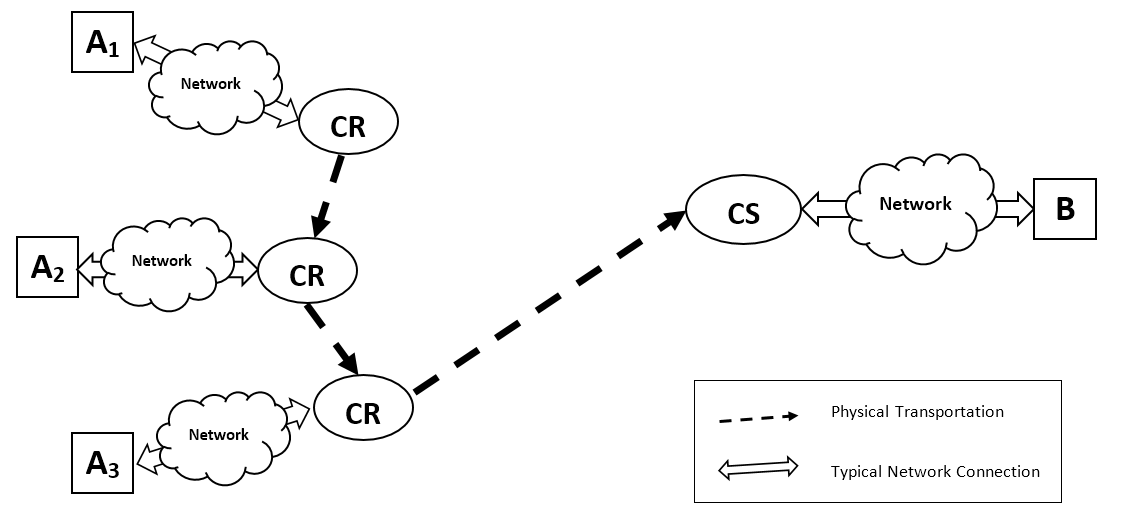
\includegraphics[width=\textwidth,natwidth=1123,natheight=530]{figures/communicationmodel.png}
\caption{Communication Model}
\end{figure}

The figure "Communication Model" illustrates the procedure of a 3-to-1 communication. The Courier first connects to A$_1$, be the role of $\mathcal{CR}$, and gets A$_1$'s message for B through the connection, then disconnects and transports to A$_2$. It should do the same thing to A$_2$ and then transport to A$_3$. After it collects all data from A$_1$, A$_2$ and A$_3$, it transports to B and be the role of $\mathcal{CS}$ to send all collected messages to B. The networks between Courier and As or B can be any kind of connection and do not to be the same, as long as both entities accept. 

To define different kinds of communication, this protocol consists of 2 sub-protocols - a) Submit protocol: how message is submitted from $\mathcal{A}$ to $\mathcal{C}$; b) Transmit protocol: after $\mathcal{C}$ gets connected with $\mathcal{B}$, how message is transmitted to $\mathcal{B}$. These two sub-protocols ensure the secure transmission of message from $\mathcal{A}$ to $\mathcal{B}$ and they will be analysed in the later part.

\subsubsection*{Behaviour Model}
Generally, all 3 entities in this protocol act as devices who possess their own initial information (described above), take $\mathcal{M}$ as input, and output $\mathcal{M'}$. All honest entities in this protocol should follow the following procedure:
\begin{enumerate}
\item If $\prod \in \mathcal{C}$, initiate the protocol by sending ${\mathcal{M}_0}'$
\item Wait for $\mathcal{M}_1$
\item Receive $\mathcal{M}_1$, decrypt all its ciphertexts and reveal their contents if applicable.
\item Check validity of the contents of $\mathcal{M}_1$ (e.g. check message format, check sender ID, receiver ID, digital signature or MAC, if applicable). If any check violates, immediately report ``Protocol Error" and abort the session.
\item Process the message content (e.g. print the result, stores the contents in local storage).
\item Prepare and send message ${\mathcal{M}_1}'$. If no message to send, abort the session silently.
\item Back to step 2.
\end{enumerate}

However, three entities have different behaviour patterns, they will be specified here, respectively:
\paragraph{Alice $\mathcal{A}$}
\begin{itemize}
\item An entity $a \in \mathcal{A}$ create the message to send, and prepare its meta data. Then it continuously listening to its network, waiting for incoming Couriers.

\item Alice will submit its message to any Courier who request for it. When submitting, the message recipient must be explicitly specified.

\item Alice is allowed to submit any message arbitrary times, to single or multiple Couriers. Alice itself should not care who carries the message, nor how many Couriers carry the message.

\item During an uncompleted session, if no response from Courier for a long time, Alice should be able to detect the timeout, cancel the effects of previous actions in this session and abort the session voluntarily.

\item If the message is not successfully sent, Alice should wait for next Couriers to send this message.
\end{itemize}

\paragraph{Bob $\mathcal{B}$}
\begin{itemize}
\item An entity $b \in \mathcal{B}$ must be continuously listening to its network, waiting for incoming messages.

\item Bob will download all messages from any Courier who transmits. If any message from $\mathcal{A}$ is invalid, Bob simply discards it.

\item Bob will discard all duplicated messages. Duplicated message are defined as messages whose Meta Signature are exactly the same. Because message Meta contains its creator ID and timestamp, same Meta reflects those messages are created by the same entity at the exact same time.

\item During an uncompleted session, if no response from Courier for a long time, Bob should be able to detect the timeout, cancel the effects of previous actions in this session and abort the session voluntarily.
\end{itemize}

\paragraph{Courier $\mathcal{C}$}
\begin{itemize}
\item As Courier's physical transportation is a very complicated task, it is out of the scope of this protocol. It is assumed that Courier is carried by an intelligent agent (such like human) who always knows where the Courier should transport to.

\item Courier should transport to every $a \in \mathcal{A}$ one by one and get their messages if there are any. Courier should be capable of storing those data for a long time.

\item After collect messages from all $a$ in the list, Courier should transport to every $b$ that is the recipient of the Courier and deliver all messages to them. If the receipt from $b$ violates the messages Courier just sent, Courier should resend the messages by restart the session again.

\item Once a full protocol run has been completed, all relative data stored in Courier is expired and should not affect future run of protocol.
\end{itemize}

\subsection*{Adversary Model}
The adversary model in this protocol is mostly derived from Dolev-Yao model which implies ``adversary carries the message" \cite{dolev}. Moreover, the adversary can also do something special in this protocol system. Specifically, adversary $\mathcal{Z}$ has following capabilities:
\begin{itemize}
\item It supervises the whole system, which means it knows when, where and how any two entities are communicating, and it knows which entity possesses what information.
\item It can access/rewrite any message passing through the network.
\item It is a legitimate user of the network and it could be any of 3 entities in this protocol.
\item It can access to all the Courier's data at any stage of the protocol.
\item Any $a \in \mathcal{A}$ or $b \in \mathcal{B}$ will always have the opportunity to be connected by any $c \in \mathcal{C}$.
\end{itemize}

It should be noted that this protocol, same as all other network protocols, is vulnerable to DoS attacks. $\mathcal{Z}$ can always prevent a message from being sent, thus it will not be covered in the security analysis.

\subsection*{Protocol Properties}
\subsubsection*{Submit protocol}
\begin{itemize}
\item $\mathcal{A}$ is authenticated to $\mathcal{CR}$
\item The Integrity of message from $\mathcal{A}$ to $\mathcal{CR}$ is preserved
\item $\mathcal{CR}$ is not able to access the message content
\item $\mathcal{A}$ is able to deny sending any message to $\mathcal{CR}$
\end{itemize}

\subsubsection*{Transmit protocol}
\begin{itemize}
\item $\mathcal{B}$ is authenticated to $\mathcal{CS}$
\item The Integrity of message from $\mathcal{CS}$ to $\mathcal{B}$ is preserved
\item $\mathcal{B}$ is able to deny receiving any message from $\mathcal{CS}$
\end{itemize}

\subsubsection*{On the whole}
\begin{itemize}
\item $\mathcal{A}$ is authenticated to $\mathcal{B}$
\item Confidentiality of message from $\mathcal{A}$ to $\mathcal{B}$ is preserved
\item Integrity of message from $\mathcal{A}$ to $\mathcal{B}$ is preserved
\item $\mathcal{A}$ can not deny sending the message to $\mathcal{B}$
\item $\mathcal{A}$ is able to deny the message content for $\mathcal{B}$
\end{itemize}

\subsection*{Property Proof}
\subsubsection*{Primitives}
Before defining the system model, all the cryptographic primitives used and their corresponding notations in this protocol should be described:
\begin{itemize}
\item Message Authentication Code $\mathcal{MAC}$\\
The MAC function used in this protocol is assumed to be secure in the sense that it has all the properties that a cryptographic hash function possesses and additionally, it resists to existential forgery under chosen-plaintext attack. That is, even if attacker is able to access an oracle which possesses the secret key and generates MACs according to the attacker's input, it is computational infeasible for attacker to guess MACs of other messages (not used to query the oracle).

\item Signature Function $\mathcal{SIGN}$\\
The signature function used in this protocol is assumed to be secure in the sense that it resists existential forgery under an adaptive chosen message attack. \cite{goldwasser}

\item Encryption Function $\mathcal{E}$ and Decryption Function $\mathcal{D}$\\
The notation $\mathcal{E}_k$ denotes an abstraction of all encryption functions, including both symmetric and asymmetric encryptions. Similarly, $\mathcal{D}_k$ represents both symmetric and asymmetric decryption functions. The subscript k denotes the key used for encryption/decryption processes.\\
To assure the security primitives of this protocol, all encryption/decryption schemes used are required to be secure in the sense that without the decryption key, it is computational infeasible for attackers to reveal the plaintext of a cipher with non-negligible probability.

\item Symmetric Key Generator $\mathcal{G}$\\
The symmetric key generator used in this protocol is assumed to be no less secure than a Cryptographically Secure Pseudorandom Number Generator. That is: \\
(a)It should satisfy the next-bit test. That is, given the first k bits of a random sequence, there is no polynomial-time algorithm that can predict the (k+1)th bit with probability of success better than 50\%. \\
(b)It should withstand "state compromise extensions". In the event that part or all of its state has been revealed (or guessed correctly), it should be impossible to reconstruct the stream of random numbers prior to the revelation. Additionally, if there is an entropy input while running, it should be infeasible to use knowledge of the input's state to predict future conditions of the CSPRNG state.\\
Furthermore, the keys generated are required to fit the Symmetric Encryption Scheme described above.
\\
(cite: from wikipedia)
\end{itemize}

\subsubsection*{Submit protocol}
\textbf{THEOREM 1:} $\mathcal{A}$ is authenticated to $\mathcal{CR}$ \\
\emph{$Proof:$} \par
Assuming $\mathcal{G}$ is secure, then $\mathcal{CR}$ is the only entity who knows the randomly generated key $k_C$. Providing $\mathcal{E}_{pk_A}$ scheme is secure, because $k_C$ is encrypted by $pk_A$ before sent out $\mathcal{A}$ will be the only entity who can reveal the encrypted $k_C$. Similarly, providing $\mathcal{MAC}$ scheme is secure, $\mathcal{A}$ is also the only one who can create MESSAGE 2 and its $\mathcal{MAC}_{k_C}$. Thus when (MESSAGE 2, $\mathcal{MAC}_{k_C}$) pair is received by $\mathcal{CR}$ and is verified true, it can be sure this message is created by $\mathcal{A}$. So $\mathcal{A}$ is authenticated to $\mathcal{CR}$.
\\
\\
\textbf{THEOREM 2:} The Integrity of message from $\mathcal{A}$ to $\mathcal{CR}$ is preserved \\
\emph{$Proof:$} \par
Assuming $\mathcal{MAC}$ scheme is secure, any modification of MESSAGE 2 will lead to unpredictable changes in the $\mathcal{MAC}_{k_C}$(MESSAGE 2) and cause its verification to be false. And according to THEOREM 1, no one else but $\mathcal{A}$ can create the message and its valid MAC, message forgery is prevented. As consequence, the message integrity is preserved.
\\
\\
\textbf{LEMMA 1} The message content cannot be revealed by any entity but $\mathcal{B}$ \\
\emph{$Proof:$} \par
Assuming $\mathcal{G}$ is secure, the randomly generated key $k_{AB}$ is only held by $\mathcal{A}$. $k_{AB}$ is encrypted by $\mathcal{E}_{pk_B}$ and sent to $\mathcal{CR}$, so assuming the $\mathcal{E}$ scheme is secure, only $\mathcal{B}$ can decrypt the cipher and reveal $k_{AB}$. As message content is encrypted by $\mathcal{E}_{k_{AB}}$, the only entity can decrypt it is $\mathcal{B}$ because only it knows $k_{AB}$ (other than the message creator). Consequently, only $\mathcal{B}$ can reveal the message content created by $\mathcal{A}$.
\\
\\
\textbf{THEOREM 3:} $\mathcal{CR}$ is not able to access the message content
\\
\emph{$Proof:$} \par
According to LEMMA 1, only $\mathcal{B}$ can reveal the message content, we can easily deduce that $\mathcal{CR}$ is not able to reveal the message content.
\\
\\
\textbf{THEOREM 4:} $\mathcal{A}$ is able to deny sending any message to $\mathcal{CR}$
\\
\emph{$Proof:$} \par
The whole message sent from $\mathcal{A}$ to $\mathcal{CR}$ contains three parts - (1) entity IDs, (2) encrypted message from $\mathcal{A}$ and (3) $\mathcal{MAC}_{k_C}$, if $\mathcal{CR}$ wants to prove the authenticity of the origin of the whole message, it must show that at least one of these three parts can be created only by $\mathcal{A}$. However, all these three parts are forgeable by $\mathcal{CR}$ itself:
\begin{enumerate}
\item entity IDs are plaintexts, thus can be created by $\mathcal{CR}$.
\item as has been proven in LEMMA 1, no entity but $\mathcal{B}$ can reveal the securely generated key $k_{AB}$, so $\mathcal{CR}$ is not able to reveal $\mathcal{SIGN_A}$ or message content, thus the encrypted message is just a block of random data for $\mathcal{CR}$, thus can be created by $\mathcal{CR}$.
\item $\mathcal{MAC}_{k_C}$ can also be created by $\mathcal{CR}$ because $\mathcal{CR}$ has $k_C$ and is able to forge the whole former message.
\end{enumerate}
To sum up, $\mathcal{CR}$ is able to create the whole message itself, it can not convince others the authenticity of the origin of the the message, so $\mathcal{A}$ is able to deny sending the message to $\mathcal{CR}$.

\subsubsection*{Transmit Protocol}
\textbf{THEOREM 5:} $\mathcal{B}$ is authenticated to $\mathcal{CS}$ \\
\emph{$Proof:$} \par
Similar to proof of THEOREM 1, providing $\mathcal{G}$ and $\mathcal{E}$ scheme are secure, only $\mathcal{B}$ knows the symmetric key generated by $\mathcal{CS}$. So, assuming $\mathcal{MAC}$ scheme is secure, if $\mathcal{MAC}_{k_C}$(MESSAGE 1) can be successfully verified by $\mathcal{CS}$, it must be $\mathcal{B}$ who create the MAC. Thus, $\mathcal{B}$ is authenticated to $\mathcal{CS}$.
\\
\\
\textbf{THEOREM 6:} The Integrity of message from $\mathcal{CS}$ to $\mathcal{B}$ is preserved \\
\emph{$Proof:$} \par
Similar to proof of THEOREM 2, any modification on MESSAGE 1 will leads to unpredictable changes in its MAC, and no one else but $\mathcal{B}$ can create the verifiable MAC of arbitrary message. So if $\mathcal{MAC}_{k_C}$(MESSAGE 1) is verified true by $\mathcal{CS}$, it means it is originally created by $\mathcal{B}$ and has not been modified. Thus the message integrity is preserved.
\\
\\
\textbf{THEOREM 7:} $\mathcal{B}$ is able to deny receiving any message from $\mathcal{CS}$ \\
\emph{$Proof:$} \par
Similar to the proof of THEOREM 4, the message from $\mathcal{B}$ is totally forgeable by $\mathcal{CS}$ because it creates the whole MESSAGE 1 and holds $k_C$, it can create $\mathcal{MAC}_{k_C}$(MESSAGE 1) by it own. Therefore $\mathcal{CS}$ cannot prove to others that the MAC is sent from $\mathcal{B}$, $\mathcal{B}$ can deny receiving any message from $\mathcal{CS}$.

\subsubsection*{On The Whole}
\textbf{THEOREM 8:} $\mathcal{A}$ is authenticated to $\mathcal{B}$ \\
\emph{$Proof:$} \par
As $\mathcal{B}$ receives two pieces of data - Meta and Msg, the authentication will be done for both of them separately.\par
\underline{Meta}: Because $\mathcal{B}$ can decrypt the encrypted Meta from $\mathcal{A}$, it can reveal the sender $\mathcal{ID}$ and $k_{AB}$, then it can further decrypt $\mathcal{E}_{k_{AB}}$($\mathcal{SIGN}_A$(Meta)) to get $\mathcal{SIGN}_A$(Meta). Assuming $\mathcal{SIGN}$ scheme is secure, if $\mathcal{B}$ verifies the signature true under $\mathcal{A}$'s public key, $\mathcal{B}$ knows Meta can only be created by $\mathcal{A}$. \par
\underline{Msg}: Assuming $\mathcal{G}$ and $\mathcal{E}$ scheme is secure, only $\mathcal{B}$ can decrypt $\mathcal{E}_{k_{AB}}$($k_{AB}$) and reveal $k_{AB}$ in Meta. Thus only $\mathcal{B}$ (other than $\mathcal{A}$) can create $\mathcal{MAC}_{k_{AB}}$(Msg). So, if (Msg, $\mathcal{MAC}_{k_{AB}}$) pair is verified true by $\mathcal{B}$, $\mathcal{B}$ knows Msg is created by $\mathcal{A}$. \par
To sum up, $\mathcal{A}$ is authenticated to $\mathcal{B}$ as all message sent by $\mathcal{A}$ is authenticated.
\\
\\
\textbf{THEOREM 9:} Confidentiality of the message from $\mathcal{A}$ to $\mathcal{B}$ is preserved\\
\emph{$Proof:$} \par
As proven in THEOREM 3, the message content from $\mathcal{A}$ to $\mathcal{B}$ can not be revealed by any other entities but $\mathcal{B}$, even the Courier itself. So after physical transportation and transmitting message to $\mathcal{B}$, this property still hold. This means only the creator and recipient of the message can reveal its content, so the confidentiality if preserved.
\\
\\
\textbf{THEOREM 10:} Integrity of the message from $\mathcal{A}$ to $\mathcal{B}$ is preserved\\
\emph{$Proof:$} \par
Similar to the proof of THEOREM 6, assuming $\mathcal{G}$ and $\mathcal{E}$ scheme is secure, $\mathcal{B}$ is the only entity who can decrypt $\mathcal{E}_{k_{AB}}$($k_{AB}$) and reveal $k_{AB}$. So when message is received by $\mathcal{B}$, only $\mathcal{A}$ and $\mathcal{B}$ hold $k_{AB}$ and are able to create $\mathcal{MAC}_{k_{AB}}$(Msg). So any forgery will lead to MAC verification fail. Further more, if the Msg is modified, it will lead to unpredictable changes in $\mathcal{MAC}_{k_{AB}}$(Msg) and fail the MAC verification as well. So if (Msg, $\mathcal{MAC}_{k_{AB}}$(Msg)) pair is verified true, the Msg must be created by $\mathcal{A}$, and remain unchanged. Thus the integrity of message from $\mathcal{A}$ to $\mathcal{B}$ is preserved.
\\
\\
\textbf{THEOREM 11:} $\mathcal{A}$ can not deny sending the message to $\mathcal{B}$\\
\emph{$Proof:$} \par
Similar to the proof of THEOREM 8, if $\mathcal{SIGN_A}$ is verified true, it proves the authenticity of the origin of the Meta, so $\mathcal{A}$ can not deny sending the message.
\\
\\
\textbf{THEOREM 12:} $\mathcal{A}$ is able to deny the message content sent to $\mathcal{B}$ \\
\emph{$Proof:$} \par
The message content contains two parts - (1) encrypted message Msg =  $\mathcal{E}_{k_{AB}}$(message) and (2) its MAC $\mathcal{MAC}_{k_{AB}}$(Msg). Because $k_{AB}$ is contained in the Meta and Meta is encrypted under $\mathcal{B}$'s public key, $\mathcal{B}$ is able to reveal $k_{AB}$. Then the whole message content part sent from $\mathcal{A}$ is forgeable by $\mathcal{B}$:
\begin{enumerate}
\item Msg is encrypted under $k_{AB}$, $\mathcal{B}$ can create any Msg it wants.
\item $\mathcal{MAC}_{k_{AB}}$(Msg) also can be created $\mathcal{B}$ because $\mathcal{B}$ can create Msg and hold $k_{AB}$.
\end{enumerate}
As $\mathcal{B}$ can create the whole content part by its own, $\mathcal{B}$ can not prove to others that the message is from $\mathcal{A}$. Thus $\mathcal{A}$ can deny the message content for $\mathcal{B}$.

\begin{thebibliography}{9}
\bibitem{goldwasser}
  Shafi Goldwasser, Silvio Micali, and Ronald Rivest,
  \emph{A digital signature scheme secure against adaptive chosen-message attacks},  SIAM Journal on Computing,
  17(2):281–308,
  Apr. 1988.
  
\bibitem{dolev}
  D. Dolev, A. C. Yao,
  \emph{On the security of public key protocols},
  IEEE trans. on Information Theory,
  IT-29: 198–208,
  1983.
\end{thebibliography}
\chapter{Protocol Implementation}
\section{Application Overview}
To run this protocol in a practical scenario, at least 3 different devices are required - one be Alice, one be Bob and one be Courier. This application implements all 3 entities within it, so once the device has this application, it can be any entity in the protocol. To achieve this, at the start of the application, user is asked to choose a particular role for the device to be. There are 4 options:
\begin{enumerate}
\item \textbf{DataCreator}, who creates message and wants to send it out.
\item \textbf{CourierReciever}, who connects to DataCreator and receives the message from it.
\item \textbf{DataReceiver}, who is the recipient of DataCreator.
\item \textbf{CourierSender}, who possesses the message from DataCreator and should transmit it to DataReceiver.
\end{enumerate}
Once the choice has been made, the graphical user interface will adjust to the selected role, and user will be requested to input some information related to the selected role. \par
Below is a snapshot of the GUI of the application, it shows all the selections and textfields that will be used when the application interacts with user.

\begin{figure}[h!]
\centering
\includegraphics[width=0.8\textwidth,natwidth=818,natheight=722]{figures/guiall.png}
\caption{GUI Overview}
\end{figure}

To run Submit Protocol, Alice should choose to run as DataCreator and Courier should choose to run as CourierReceiver. Then Courier transports to Bob and chooses to run as CourierSender, meanwhile Bob should choose to run as DataReceiver to run Transmit Protocol with Courier. The detailed instruction of how to run those two sub-protocols is given in the appendix. \par

To further illustrate how user can interact with the system, a use case diagram is given and every use cases appear in the diagram will be explained. For disambiguating, the ``Alice", ``Bob" and ``Courier" appeared in the use case diagram do not mean the protocol entity as introduced in the system model, but are the names of the actors who control the device. The name of the actor simply reflects which entity the actor wants to be in the protocol. \\

\begin{figure}[h!]
\centering
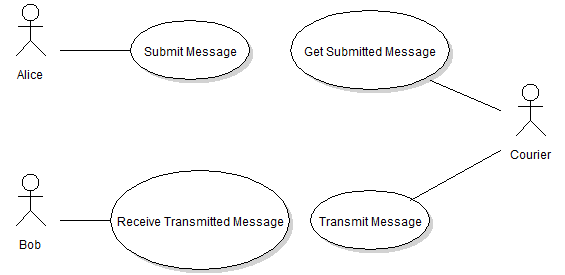
\includegraphics[width=0.6\textwidth,natwidth=565,natheight=275]{figures/usecasediagram.png}
\caption{Use Case Diagram}
\end{figure}

\subsection*{Use Case 1: Submit Message}
\begin{tabular}{|l|p{0.6\textwidth}|}
 \hline
 Title & Submit Message \\ \hline
 Primary Actor & Alice \\ \hline
 Goal in Context & Alice tries to submit the message to a Courier \\ \hline
 Scope & System (Black Box) \\ \hline
 Level & \\ \hline
 Stakeholders & Alice and Courier \\ \hline
 Success Guarantees & Message is received by Courier and Alice confirms the fact \\ \hline
 Trigger & Alice starts the Submit Protocol \\ \hline
 Main Success Scenario & 
 \parbox{9cm}{
  \medskip
  1. Alice starts the application. \\
  2. Alice selects ``DataCreator" as the protocol entity in the application. \\
  3. Alice specifies all related information as instructed in the ``Run Submit Protocol" section in Appendix A: User Manual. \\
  4. Alice starts running the protocol.
  \medskip
 }
 \\ \hline
\end{tabular}
\\
\\
\subsection*{Use Case 2: Get Submitted Message} 
\begin{tabular}{|l|p{0.6\textwidth}|}
 \hline
 Title & Get Submitted Message \\ \hline
 Primary Actor & Courier \\ \hline
 Goal in Context & Courier tries to obtain the message of Alice \\ \hline
 Scope & System (Black Box) \\ \hline
 Level & \\ \hline
 Stakeholders & Courier and Alice \\ \hline
 Success Guarantees & Courier gets a message from Alice \\ \hline
 Trigger & Courier starts the Submit Protocol \\ \hline
 Main Success Scenario & 
 \parbox{9cm}{
  \medskip
  1. Courier starts the application. \\
  2. Courier selects ``CourierReceiver" as the protocol entity in the application. \\
  3. Courier specifies all related information as instructed in the ``Run Submit Protocol" section in Appendix A: User Manual. \\
  4. Courier starts running the protocol.
  \medskip
 }
 \\ \hline
\end{tabular}
\\
\\
\subsection*{Use Case 3: Receive Transmitted Message} 
\begin{tabular}{|l|p{0.6\textwidth}|}
 \hline
 Title & Receive Transmitted Message \\ \hline
 Primary Actor & Bob \\ \hline
 Goal in Context & Bob tries to receive message of Alice carried by Courier \\ \hline
 Scope & System (Black Box) \\ \hline
 Level & \\ \hline
 Stakeholders & Bob and Courier \\ \hline
 Success Guarantees & Bob receives the message \\ \hline
 Trigger & Bob starts the Transmit Protocol \\ \hline
 Main Success Scenario & 
 \parbox{9cm}{
  \medskip
  1. Bob starts the application. \\
  2. Bob selects ``DataReceiver" as the protocol entity in the application. \\
  3. Bob specifies all related information as instructed in the ``Run Transmit Protocol" section in Appendix A: User Manual. \\
  4. Bob starts running the protocol.
  \medskip
 }
 \\ \hline
\end{tabular}
\\ 
\\
\subsection*{Use Case 4: Transmit Message}
\begin{tabular}{|l|p{0.6\textwidth}|}
 \hline
 Title & Transmit Message \\ \hline
 Primary Actor & Courier \\ \hline
 Goal in Context & Courier tries to transmit Alice's message to Bob \\ \hline
 Scope & System (Black Box) \\ \hline
 Level & \\ \hline
 Stakeholders & Courier and Bob\\ \hline
 Success Guarantees & Message is received by Bob and Courier confirms the fact \\ \hline
 Trigger & Courier starts the Transmit Protocol \\ \hline
 Main Success Scenario & 
 \parbox{9cm}{
  \medskip
  1. Courier starts the application.
  2. Courier selects ``CourierSender" as the protocol entity in the application.
  3. Courier specifies all related information as instructed in the ``Run Transmit Protocol" section in Appendix A: User Manual.
  4. Courier starts running the protocol.
  \medskip
 }
 \\ \hline
\end{tabular}
\\

\section{Software Design}
The implementation of this protocol mainly consists of two parts - a core library and an user interface. The core library defines the framework of the program and provides all essential components for running the protocol. While the user interface takes user's input, configures components provided by the core library, runs the protocol and outputs running results if necessary. This design separates the implementation of user interfaces from the actual running of the protocol, the major benefit is that when this protocol is running on different devices or platforms, its user interfaces can be customized and easily plugged to the core library without modifying it.

\subsection{Program Architecture}
As introduced above, the whole program contains 4 roles - DataCreator, DataReceiver, CourierSender and CourierReceiver. Classfied by their main structure, those 4 different roles fall into 2 categories - (1) Accepter, who continuously listens to the port and waits for incoming connection. (2) Initiator, who actively connects to a Accepter. Although these two categories sounds similar to Client-Server pattern, it is not quite the case because Accepter does not actually provide any service. Based on their behaviour definition in protocol specification, DataCreator and DataReceiver belong to Accepter, while CourierSender and CourierReceiver belong to Initiator. Following paragraphs will introduce the internal architecture for Accepter and Initiator respectively.
\paragraph{Accecpter}
Accepter contains 5 main parts:
\begin{itemize}
\item Dispatch Thread \\
The Dispatch Thread listens to the program port, waits for incoming connections. Once it receives a connection, it will create a new session, then handover the connection to the newly created session. After that, it will continue listening to the port, wait for next incoming connection.

\item Sessions \\
Sessions are created by the Dispatch Thread, each session corresponds to a single connection and sessions are independent between each other. Once a session takeovers a connection, it is fully responsible for it. Inside a session there is a Delegate and a Sub-thread. 
\par The \textbf{Delegate} defines all communication content (e.g. a Delegate of Alice defines the content of messages to send out, and it also defines what to do when receives a certain message), it behaves like a state machine which takes message as input, processes the message and output a new message for response. During the processing of input messages, it may interact with the 3 global objects - User Interface, Cryptographic Kit and Data Manager. The detail of Delegate will be explained in Delegate Model.
\par The \textbf{Sub-thread} listens to the connection which is handover by Dispatch Thread, capture any message from the connection. It delivers the captured message to Delegate, and receives a new message from Delegate. If the output message from Delegate does not indicate an exception or termination, the Sub-thread sends the message through the connection, otherwise it reports an error or terminates.

\item User Interface \\
The User Interface is shared between all sessions in Accepter. It displays all relative information to show the progress of the protocol running and reports errors to the user.

\item Cryptographic Kit \\
The Cryptographic Kit is shared between all sessions in Accepter. It provides functionalities of all cryptographic operations that is needed in the protocol, such as encryption, decryption, key generation, MAC generation and verification, and digital signature generation and verification. When any session need to do cryptographic operations, it just call from Cryptographic Kit and doesn't care the internal implementation. For the consistency concern, it is required that any two communicating device should use same Cryptographic Kit.

\item Data Manager \\
The Data Manager is shared between all sessions in Accepter. It keeps record of all data files in the device's disk which is related to the protocol, such as files of public keys, secret keys, and the message Courier carries. Data Manager is configured at the start of the application, when any session need data in disk, it just request from Data Manager.
\end{itemize}
The relation between those 5 components is illustrated in the figure ``Accepter Architecture".

\begin{figure}[h!]
\centering
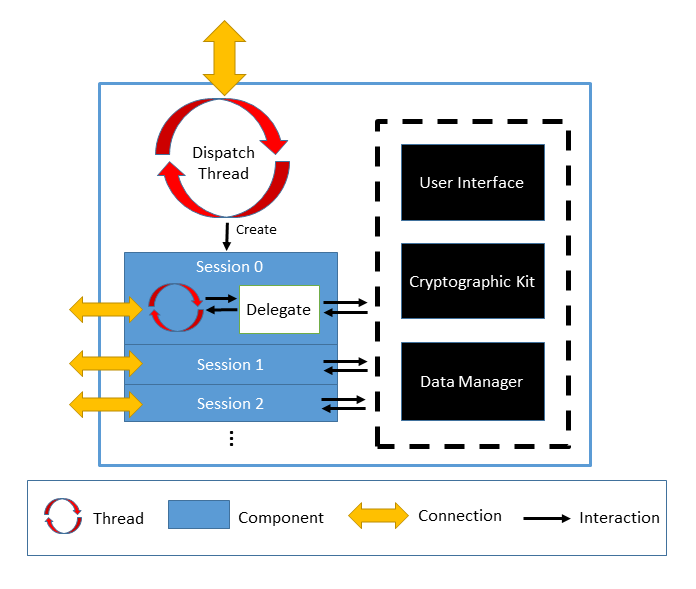
\includegraphics[width=\textwidth,natwidth=696,natheight=589]{figures/accepterarchitecture.png}
\caption{Accepter Architecture}
\end{figure}

\paragraph{Initiator}
Similar to Accepter, Initiator consists of 4 main parts: (1) Session, (2) User Interface, (3) Cryptographic Kit and (4) Data Manager. The major difference between Initiator and Accepter is that Initiator does not have a Dispatch Thread, every Initiator only has one Session. The Session is created once the Initiator is started, and it will ask its Delegate for a ``initial message" - which will be the first message of the protocol, and will be sent to the specified Accepter. The architecture design of Initiator is a simpler version of Accepter's, and it is illustrated in the figure ``Initiator Architecture".

\begin{figure}[h!]
\centering
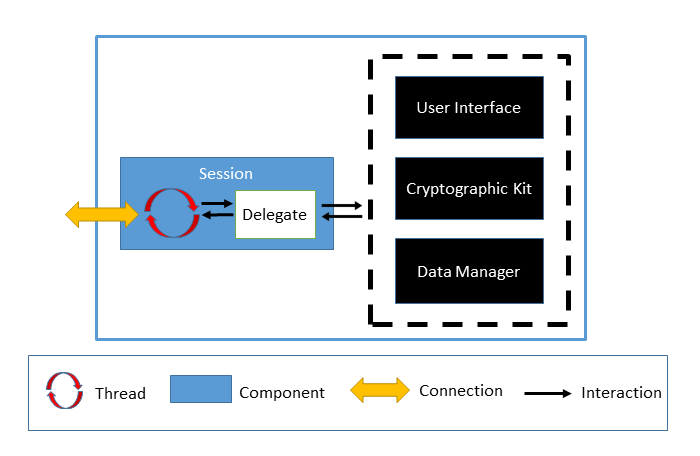
\includegraphics[width=\textwidth,natwidth=700,natheight=456]{figures/initiatorarchitecture.png}
\caption{Initiator Architecture}
\end{figure}

\subsection{Delegate Model}
The object Delegate is the essence of the application, it directly refers to the specification of the protocol, defines how an entity processes a message - here ``process a message" may involve doing cryptographic operations, checking message content validity and giving a response message.

Basically, every Delegate acts like a finite-state machine, who possesses an internal state, takes messages as inputs and outputs new messages as response. The internal state controls the behaviour of the Delegate - Delegates in different states will respond differently to a same input. So when an input message comes, Delegate will process the message according to its current state, if the message is successfully processed, it will change its current state and wait for next message, until it reaches the final state. 

Taking entity $\mathcal{A}$ as example,the figure below shows a 4-internal-state machine which abstracts the behaviour of $\mathcal{A}$: initially $\mathcal{A}$ is in Wait state, waiting for the first message. Once it receives the first message, it will process the message (according to the Submit Protocol, it will check the first message and submit its data to Courier). If $\mathcal{A}$ successfully processed M$_0$, it enters Submitted state, waiting for the second message. Then it will receive and process M$_1$ (according to the Submit Protocol, it will check the validity of the MAC).  If it is successful again, it enters the final state Checked and stops. If any error occurs in processing the input messages in early states, $\mathcal{A}$ directly enters final state Error and stops.

\begin{figure}[h!]
\centering
\includegraphics[width=0.8\textwidth,natwidth=585,natheight=352]{figures/statemachinefigure.png}
\caption{State Machine of $\mathcal{A}$}
\end{figure}

\subsection{Message Structure}
Based on the protocol specification, there are totally 5 different kinds of messages to exchange in a single success protocol run - 3 messages are needed to achieve Submit Protocol and 2 messages are needed to achieve Transmit Protocol. The design of message structure attempts to maximize the time efficiency of the protocol, thus no extra message will be exchanged and the lengths of messages will be minimized. All messages exchanged in this protocol are concatenations of 6 different kinds of primary blocks:
\begin{itemize}
\item \textbf{Integer Block} \\
Integer Block simply contains a single Integer, it occupies 4 bytes (based on the current JAVA's Implementation).

\item \textbf{MAC Block} \\
MAC Block contains a cryptographic MAC, whose size is defined by the Cryptographic Kit the application uses.

\item \textbf{Asymmetric Cipher Block} \\
Asymmetric Block contains an asymmetric cipher. Because encrypting a long plaintext using asymmetric encryption takes long time, to reduce the computational consumption, the length of plaintext for asymmetric encryption is restricted in this protocol, so that only one cipher block will be produced after the encryption. As the consequence, the size of Asymmetric Cipher Block is fixed, which is 128 bytes (based on a key of size 128 bits).

\item \textbf{ID Block} \\
ID Block contains two parts. The front part is a single byte which indicates the total length of the ID string and the following part is a string of characters representing the ID. The size of ID Block is variable, which is the length of ID string plus 1 bytes.

\item \textbf{Meta Block} \\
The Meta Block in application design is different with ``Meta block" in protocol specification. It contains a concatenation of 3 parts - (1) an integer indicates the size of the rest of this Meta Block, (2) an asymmetric cipher of the meta of the message, (3) a symmetric cipher of the signature of the meta. As explained in Asymmetric Cipher Block, the size of all asymmetric ciphers is fixed, so the size of the asymmetric cipher is (size of Meta Block - size asymmetric cipher).

\begin{figure}[h!]
\centering
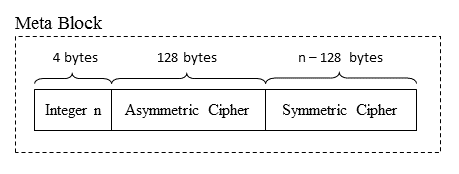
\includegraphics[width=0.6\textwidth,natwidth=459,natheight=174]{figures/metablock.png}
\caption{Structure of Meta Block}
\end{figure}

\item \textbf{Message Block} \\
The Message Block is also different with ``Msg block" in protocol specification. Similar to Meta Block, it is the concatenation of 3 parts - (1) an integer indicates the size of the rest of this Message Block, (2) a symmetric cipher of the actual message content, (3) a MAC of the part (2). The size of symmetric cipher can also be deduced as the size of MAC is fixed.

\begin{figure}[h!]
\centering
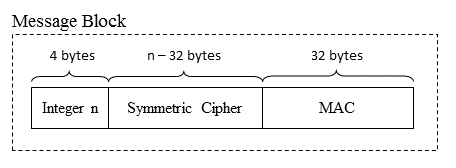
\includegraphics[width=0.6\textwidth,natwidth=456,natheight=168]{figures/messageblock.png}
\caption{Structure of Message Block}
\end{figure}
\end{itemize}

To summarize, 3 of these 6 primary blocks are fixed-size blocks (Integer Block, MAC Block and Asymmetric Cipher Block), while other 3 of them are variable-size blocks (ID Block, Meta Block and Message Block). All the messages exchanged in the protocol are constructed by these primary blocks through concatenation, and they will be illustrated below.

\subsubsection*{Submit Protocol}
Message 1, from Courier to Alice: \\
\begin{tabular}{|c|c|c|}
 \hline
 ID Block & Integer Block & \qquad\; AC Block \qquad\; \\ \hline
\end{tabular}

\noindent\bigskip
\textit{Note that ``AC Block" denotes Asymmetric Cipher Block.}

\noindent
Message 2, from Alice to Courier: \\\bigskip
\begin{tabular}{|c|c|c|c|c|}
 \hline
 ID Block & ID Block & \qquad\; Meta Block \qquad\; & 
 \quad\, Message Block \quad\, & MAC Block \\ \hline
\end{tabular}

\noindent
Message 3, from Courier to Alice: \\\bigskip
\begin{tabular}{|c|c|c|}
 \hline
 MAC Block \\ \hline
\end{tabular}

\subsubsection*{Transmit Protocol}
Message 1, from Courier to Bob: \\
\begin{tabular}{|c|c|c|c|c|c|}
 \hline
 ID Block & \qquad\; AC Block \qquad\; & 
 \; Meta$_0$ \; & Message$_0$ & 
 \; Meta$_1$ \; & Message$_1$
 \\ \hline
\end{tabular}
\textbf{......} \\
\noindent\bigskip
\textit{Multiple Meta Blocks and Message Blocks can be appended here.}

\noindent
Message 2, from Bob to Courier: \\\bigskip
\begin{tabular}{|c|c|c|}
 \hline
 MAC Block \\ \hline
\end{tabular}

\subsubsection*{Error Message Flag}
There are two kinds of messages exchanged in the protocol, all above messages are one of them, called Normal Message, the others called Error Message. Those two kinds of messages are distinguished by an Error Message Flag, which is the first byte of the message. Thus there is an extra step before above Normal Messages to be sent - they should be wrapped by an extra byte 0 at the front of them. While an Error Message contains two parts - (1) a byte indicates the size of the rest of the message, (2) a string of error information. As consequence, all messages start with a byte 0 will be treated as Error Message. The figure below further illustrates the difference between Normal Message and Error Message.

\begin{figure}[h!]
\centering
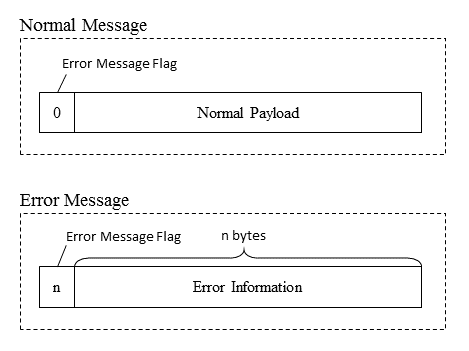
\includegraphics[width=0.6\textwidth,natwidth=469,natheight=351]{figures/normalvserrormessage.png}
\caption{Normal Message and Error Message}
\end{figure}

\section{Implementation Details}
\subsection{UML Class Diagram}
A UML Class Diagram has been plotted to show all the main classes in the program and the relations between them.
\begin{figure}[h!]
\centering
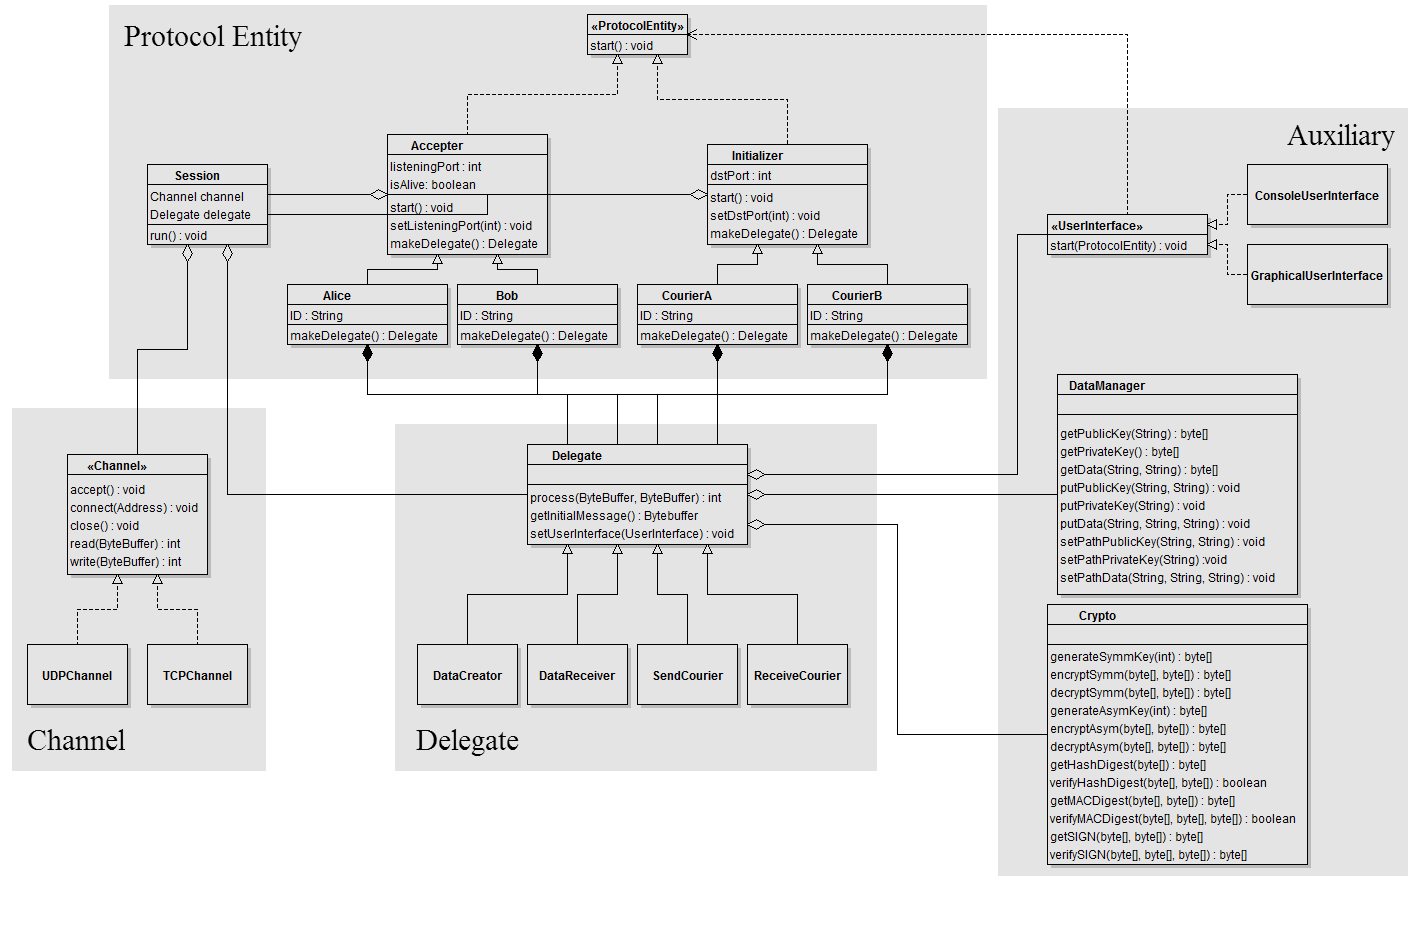
\includegraphics[width=\textwidth,natwidth=1416,natheight=935]{figures/umldiagram.jpg}
\caption{UML Diagram}
\end{figure}

According to the diagram, the whole program can be separated into 4 main parts:
\begin{itemize}
\item \textbf{Protocol Entity} \\
This part defines the framework of this application. Any protocol entity can be first specified into an Accepter or an Initiator, then based on the role it plays, it can be further classified into a particular role like Alice, Bob, CourierA (Courier who connects to Alice) or CourierB (Courier who connects to Bob). As shown in the diagram, every level of classification corresponds to a group of classes and lower level classes inherit from the higher level classes. The main job of Protocol Entity classes is creating, initializing and managing its Session objects. While a Session class - which is possessed by every protocol entity, deals with the message transmission issues for the entity, such as requesting next messages from Delegate, sending messages to the Channel, etc.

\item \textbf{Channel} \\
The Channel is used in Session class, it is an Interface denotes a place where messages can be sent and received. Ideally, when two channels are connected, devices can easily push message in and receive message from their channels without awareness of any detail about the connection. However, due to different networks and protocols suites may be used when running CDSProtocol, various implementations of Channel are necessary. As shown in the diagram, possible implementations of Channel Interface can be TCPChannel and UDPChannel, corresponds to connecting under TCP or UDP. Except above two, even more different channels could be developed like BluetoothChannel, CableChannel, etc. In this prototype program, only UDPChannel is currently implemented and the detail of it will be explained in the later ``Connection Establishment" section.

\item \textbf{Delegate} \\
As has been demonstrated in the ``Delegate Model", Delegate class defines the ``rule" of an entity. It takes a message as input, processes the message and outputs a responding message if there is one. However, Delegate is just an abstract notion, its children classes define the real ``rules" of each entity respectively. As shown in the diagram, DataCreator, DataReceiver, CourierSender, CourierReceiver are 4 different implementations of Delegate class, they define the ``rules" for the 4 entities correspondingly - Alice, Bob, CourierA and CourierB.

\item \textbf{Auxiliary} \\
This part contains 3 components that can be totally independent with the design of CDSProtocol. The UserInterface only deals with inputs from user and displays output to user. Reflect to the software design, its implementation can be various to fit different devices and platforms. The DataManager takes charge of managing the disk files that is related to the running of the protocol. And the Crypto represents ``Cryptographic Kit" in the software design, its job is to provide all cryptographic operations that is needed in the protocol.
\end{itemize}

\paragraph{Extensibility and Reusability}
The design of the program structure attempts to maximize the extensibility and reusability of the program in order to make the program easy for modifying and extending after release. It should be noticed that all components of the program are loosely coupled which makes them easy for reuse, and frequently used inheritance and interfaces makes the program extensible. Developers can modify or create their own entities, delegates, channels or even cryptographic kits without affecting other parts of the code. 

\subsection{Connection Establishment}
The Channel is used to establish connections between entities in program. Each Channel object is associated with a local address and listening port before connected. There are 2 steps for two entities to get connected using Channel. Firstly, Initiator initiates the connection by calling the connect() method of its Channel object, specifying the destination IP address. Then the Accepter accepts the connection by calling the accept() method of its Channel object. The accept() method will wait until there is a connection to accept and what it really does is creating a new Channel object which is connected to the incoming connection, and returns that newly created Channel object. Once the connection is accepted, both entities can use Channel's read() and write() method for receiving and sending messages. If any of the entity chooses to terminate the connection, it calls the close() method of its Channel, then both Channels are closed.

\paragraph{UDPChannel}
The above connecting mechanism is effective in this protocol, as the Channel object who accepts connections will not be connected to any Channel, thus it can accept several connections without changing its listening port - imaging if channel gets connected once it accepts a connection, then when a new connection comes, it will not be able to accept it. However, to implement this mechanism for UDP requires extra effort because UDP itself is connectionless and every packet sent or received is independent between each other. The real process for establishing connections using UDPChannel is: When the Initiator calls the connect() method of its Channel object, the channel records the destination address and port number but sends nothing. So when Accepter calls accept() nothing will happen until Initiator sends the first message, at which point accept() will create a new Channel object with a different listening port and all future messages will be sent through this Channel object. So, when Accepter sends back the second message, the port number of the channel sending the message is different with what Initiator specified in the first message. So when Initiator receives a reply message fron Accepter, it changes its channel's destination port number to the coming channel's port number, so that its future messages will be sent to the Accepter's newly created channel. Finally the connection is built between Initiator's channel and Accepter's newly created channel.

\subsection{Message Processing}
When a message is received from the channels, it will be examined by the session first, where the Error Message Flag will be checked. If the Error Message Flag (the first byte of the received message) is greater than 0, it indicates the message is an Error Message and the number of the Error Message Flag represents is the length of the error information. Then session will extract the error information and displays it on the user interface. If the Error Message Flag is 0, it means the message is a Normal Message. Then session will extract the payload and feed it to the delegate. Delegate will further process the payload and returns an integer indicating the size of the responding message. If the integer is 0 it means the message is successfully processed and no further messages to be sent. If the integer is negative, it means an exception occurs during the processing.

When session gets a message from delegate, it should wrap it into a Normal Message by adding a 0 byte in the front of the message. Then session sends the wrapped message to the channel and waits for receiving next message from the channel.

\subsection{Cryptographic operations}
The cryptographic functions provided by the Crypto class in this program are mainly built from two Java packages ``java.security" and ``javax.crypto", thus the security of this application highly relies on the implementation inside those two Java packages. Below will list and explain all the cryptographic operations used in this protocol. As there is no sign indicating there is any flaw inside the Java security packages, we will not dig too deep into the security cryptographic implementation. 

\begin{itemize}
\item \textbf{Symmetric Encryption / Decryption / KeyGeneration} \\
The symmetric encryption / decryption scheme used is AES \cite{Miller}. The mode of operation used is CBC \cite{ehrsam1978message}. The padding scheme is PKCS\#5 \cite{RFC2898}. The size of key used is 128 bits and it should not exceed 936 bits.

\item \textbf{Asymmetric Encryption / Decryption / KeyGeneration} \\
The asymmetric encryption / decryption scheme used is RSA. The mode of operation used is ECB, however, for efficiency concern, the size cipher block of asymmetric encryption will be restricted to 1, so mode of operation will not actually be used in the program. Th padding scheme is PKCS\#1 \cite{RFC2313}. The size of key used is only 1024 bits, as this is only a prototype application and key size can easily be increased in future.

\item \textbf{MAC Creation / Verification} \\
The MAC algorithm used is Hmac-SHA-256 \cite{RFC6234}. The size of key used is same to symmetric encryption / decryption, which is 128 bits.

\item \textbf{Digital Signature Creation / Verification} \\
The signature algorithm used is RSA. The cryptographic hash function used in SHA256 \cite{RFC6234}. They key size is same to asymmetric encryption / decryption, which is 1024 bits.
\end{itemize}

\subsection{File Management}
It is assumed that adversary is not able to hack into its target entity's system, that is, the adversary can not access to the memory or disk of a honest entity's device. Based on this assumption, all the data files are stored explicitly in device's disk.
\paragraph{Keys}
As a single device is able to act as several different entities, it is possible that one device possesses several secret keys and presumably a long list of others' public keys. The user should take care of his/her own key files, and before the protocol starts, he/she specifies the locations of all keys. Then during running, the application will read those files when necessary.
\paragraph{Alice's Message Content}
Similar to the keys, Alice's message content should be stored in the disk of Alice's device. Before the start of the protocol, user will be requested to specify the location of that file. Then during Submit Protocol, the file will be read when necessary.
\paragraph{Courier's Payload}
Courier's payload files are not specified by user, it is managed by the application. For every Courier entity, it has a working directory, by default, Courier's working directory is in the application's directory, named after its ID. Once Courier gets data from Alice in Submit Protocol, it will save the data into its working directory, the file name will be the destination entity's ID. For example, if Courier0 receives data from Alice to Bob, the data will be saved in the file ``./Courier0/Bob". As Courier may receives data from multiple datacreators, all further data will be appended to the file named after the receiver's ID, if no such file, program will create it. So, after the Message Acquisition phase, Courier may have several data files, and each contains data from multiple datacreators. Finally in Transmit Protocol, Courier transmits the corresponding data file to its destination entity base on the file name.

\subsection{Error Handling}
In this application, errors are classified into 4 main classes - user input error, I/O error, protocol error and timeout. Below will explain the details of these 4 errors and how they are handled in the program.
\paragraph{User Input Error}
User input errors occur when user input meaningless content into the application's textfield, such as inputing non-numeric string as port number, etc. This kind of errors will be caught before the protocol starts running, after user click ``Start" button. Once user input error is detected, its detail will be sent to user interface where the error detail will be shown to the user.
\paragraph{I/O Error}
I/O error denotes errors happening when reading/write files or sending/receiving through network channels, such as files not found when reading files, or port number is in use when creating a network socket, etc. These errors are caught during the running of the protocol and will cause termination of the protocol run. Similar to user input error, once I/O error is detected, its detail will be sent to user interface and then be shown to the user.
\paragraph{Protocol Error}
Protocol error is produced by the protocol itself, when there is some checking violation happens such as verifying a MAC to false, or the message size exceeds the capacity of Courier's storage, etc. All the checking processes have been fully described in the protocol specification, and the program strictly follows those processes. Because all checking operations happen in delegates while delegates processing the received messages, the protocol error is detected by delegates. Once a protocol error is detected, firstly, the error detail will be sent to user interface and be shown to the user. Meanwhile, the delegate will return a negative integer indicating error happens during processing. Then session will send a Error Message to the other entity reporting the error. However, for the security concern, Error Message will not include any detail about the error, currently it just carries a string ``Protocol Error".
\paragraph{Timeout}
Technically timeout is not an error but a mechanism of protecting an entity from waiting responses for too long time. And it is essential in this protocol because when an I/O error occurs during the protocol, it immediately terminates the program in this device, without reporting anything to the other device which still waits for reply. Timeout allows the other device to abort the protocol if no message is received after waiting for a certain amount of time. Timeout is detected in sessions. After sending out a message session will first check whether it is the end of the protocol, if it is, session will close the channel and terminate. If it is not, session will monitor the channel with a timer. Upon the time runs out, it will voluntarily close the channel and terminate.
\chapter{Test and Evaluation}
In this chapter, several performance tests will be done to the program developed for running CDSP. As there is no any other existing program developed for CDSP, the test results will not be compared to any others. The main purpose of these performance tests is to show the efficiency of the current implementation of CDSP so that it can be taken as a point of reference for future development.

The rest of the chapter will first describe the system environment that is used for the testing. Then tests results will be given for both Submit Protocol and Transmit Protocol separately. For each sub-protocol, two main kinds of test are done - latency test and scalability test. Finally a summary will conclude the testing result for both Submit and Transmit Protocol.

\section{Test Environment}
Following is a snapshot of the system environment used for the testing:\\

\noindent
\begin{tabular}{|l|p{0.6\textwidth}|}
 \hline
 Processor & Intel\textregistered \space Core\texttrademark \space i7-3610QM CPU @ 2.30GHz $\times$ 4 \\ \hline
 Installed Memory & 8 GB \\ \hline
 OS Platform & Ubuntu 12.04 LTS \\ \hline
 OS Type & 64-bit \\ \hline
 Network Interface & Loopback \\ \hline
 JRE Version & 1.7.0\textunderscore07 - b11 \\ \hline
\end{tabular}\\
\bigskip

\noindent
To eliminate the influence of various UI implementations, a UI called ``NullUserInterface" is used in the testing. In ``NullUserInterface", all parameters required from user input are all hard-coded thus it can be run automatically by only using commands. On the other hand, ``NullUserInterface" does not produce any output for user, it only outputs the testing results to the terminal so no extra computational resource will be used in dealing with outputs during the test.

\section{Submit Protocol}
\subsection{Latency Test}
The latency here refers to the total time cost for successfully running Submit Protocol once. It is defined as the time cost from the point that Courier initiates a connection to the point that Courier sends out the message 3 (a MAC as receipt confirmation). There are two reasons for defining the end point as Courier sending message 3, but not Alice receives message 3 : (1) It is very difficult to coordinate different times of two entities, especially in millisecond scale. (2) After Courier sends out message 3, it will leave immediately without caring whether the message will be received or not, and no further action of Courier depends on the arrival of message 3. Thus it is reasonable to define the sending of message 3 as the end of the Submit Protocol. 

The test programs contains running of two entities:
\begin{enumerate}
\item An Alice continuously listens to the port and is ready to start the Submit Protocol.
\item A Courier initiates the Submit Protocol, and once it sends out a message 3, it immediately creates another Courier and initiates the protocol with Alice again. This process repeats for 1000 times.
\end{enumerate}
The system records the time cost from the beginning of the program to Courier running the 100th, 200th, 300th,... 1000th times of the protocol respectively. The message content Alice sends is a 18 bytes string.

\begin{figure}[h!]
\centering
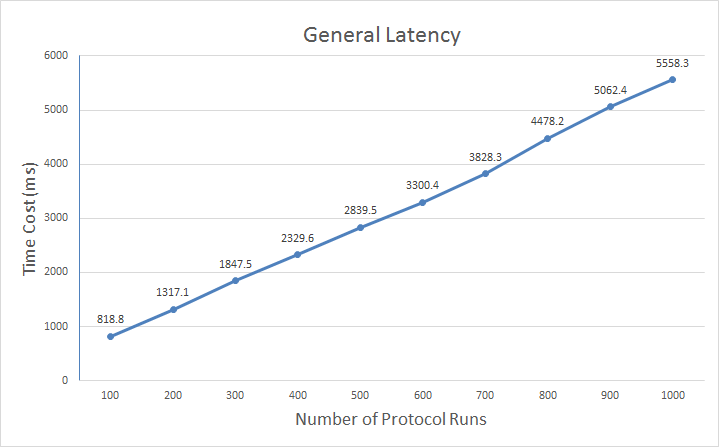
\includegraphics[width=0.7\textwidth,natwidth=719,natheight=447]{figures/latencysubmit.png}
\caption{General Latency Test of Submit Protocol}
\label{fig:latencysubmit}
\end{figure}

The test is done for totally 10 times and the final result is the average number of each testing result. Figure~\ref{fig:latencysubmit} shows the final result. Through the chart we can see the latency grows linearly with the number of communications - which is expected. And figure~\ref{fig:averagelatencysubmit} shows the average latency for every protocol run. The chart indicates that when the number of consecutive communication grows large, the average latency for each communication becomes stabilized around 5.5 milliseconds. In practice, there might be hundreds of entities within the system, a single message creator may send thousands of messages in a short period of time, and above result just proved that a single message creator is able to sequentially complete 1000 of message sending tasks around 5.5 seconds. This outcome is satisfying. 

\begin{figure}[h!]
\centering
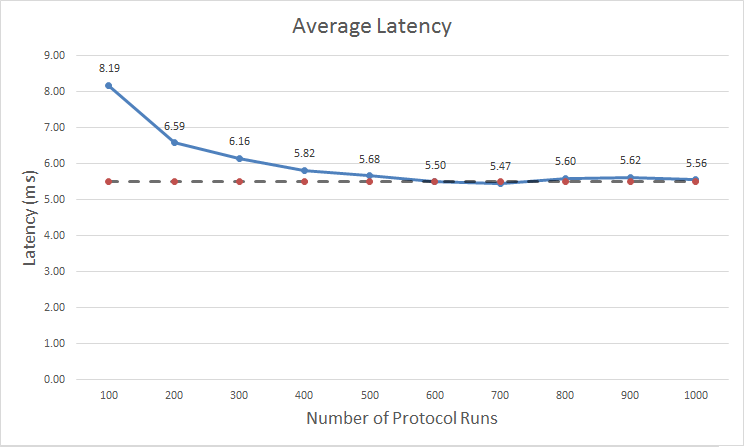
\includegraphics[width=0.7\textwidth,natwidth=744,natheight=447]{figures/averagelatencysubmit.png}
\caption{Average Latency of Submit Protocol}
\label{fig:averagelatencysubmit}
\end{figure}

\subsection{Scalability Test}
To thoroughly show the scalability of Submit Protocol, the performance of the protocol will be measured under two conditions - the growth of message size and the growth of communicating entities. Their methodologies and analysis results will be given separately below.

\subsubsection{Scale of Message Size}
In this test, it is expected to reveal how Submit Protocol will behave when the size of message to be sent increases.

The programs used are same with above latency tests - a normal message creator and a courier who repeatedly initiates Submit Protocol with the message creator.

The system records the latency of 1000th successful run of Submit Protocol with different sizes of messages. The message sizes are various from 1 byte to 10 KB. To make the test more convincing, we collect 5 data samples for every message size, and the result is plotted in a scatter chart figure~\ref{fig:messagesizesubmit}. The chart shows the total latencies for submitting 1000 times 1 Byte, 10 Bytes, 100 Bytes, 1 KB, 2 KB, 3KB, 4KB, 5KB and 10 KB messages respectively. It is shown that compare to the dramatical increasing extent of message size, the rise of latency is quite subtle - from around 5500 milliseconds to around 6200 milliseconds while message size is 10000 fold! Furthermore, following the trend line in the chart, it can also be observed that the grow trend of latency is linear which is ideal for the protocol.

\begin{figure}[h!]
\centering
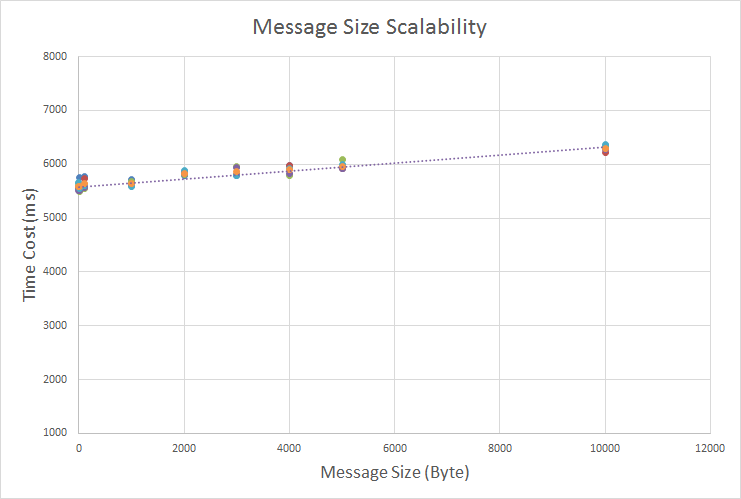
\includegraphics[width=0.7\textwidth,natwidth=741,natheight=499]{figures/messagesizesubmit.png}
\caption{Latency with Message Size for Submit Protocol}
\label{fig:messagesizesubmit}
\end{figure}

Using the same data sample, we can also calculate the relationship between the throughput and message size. We define the notion ``effective throughput" as the size of actual message content being sent per second. Namely, it does not count those extra bits which are the overhead for delivering the message. It represents the efficiency of the protocol in terms of delivering messages contents. Figure~\ref{fig:effectivethroughputsubmit} illustrates how the effective throughput of Submit Protocol changed when the message size increased. As the chart shows, the correlation between effective throughput and message size is linear, which is a good news because it means that the larger the messages are the more effective the protocol is. And when the message size increased to 10 KB, the effective throughput reaches nearly 1.6 MB/s. Of course, the effective throughput will not keep increasing infinitely, it will eventually hit the ceiling and restricted by the network throughput and capability of devices' available memory, however as 10 KB size is already considered very large for a single message, the efficiency at this level is good enough.

\begin{figure}[h!]
\centering
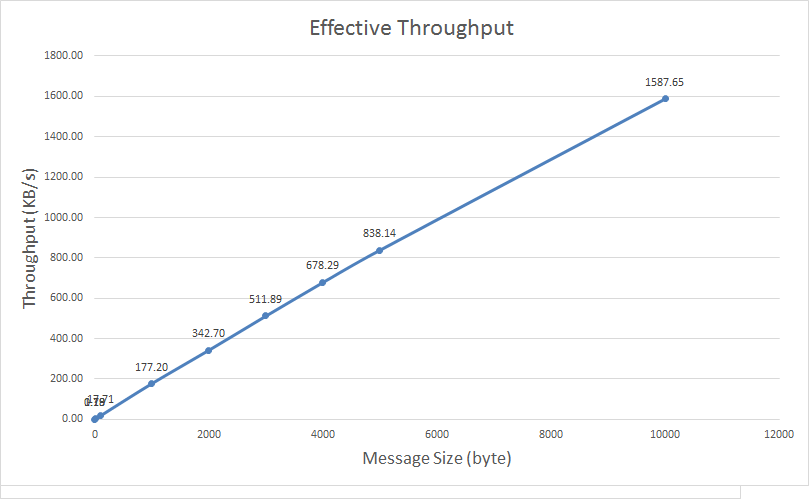
\includegraphics[width=0.7\textwidth,natwidth=809,natheight=499]{figures/effectivethroughputsubmit.png}
\caption{Effective Throughput with Message Size for Submit Protocol}
\label{fig:effectivethroughputsubmit}
\end{figure}

\subsubsection{Scale of Concurrent Communication}
In practice, it is highly probable that a single message creator will submit messages to several couriers simultaneously, this test reflects this scenario and aims to show the behaviour of Submit Protocol under the situation where concurrent communication is involved.

The testing program contains 3 entities:
\begin{enumerate}
\item An Alice continuously listens to the port and is ready to start the Submit Protocol.
\item A noisy Courier initiates the Submit Protocol with Alice, and once it sends out a message 3, it immediately creates another noisy Courier and initiates with Alice again. This process repeats for 100 times. It records the time cost for running 100 times of the protocol and yield the result.
\item Several silent Couriers initiate the Submit Protocol with Alice along with the noisy Courier. Same with noisy Courier, every silent Courier repeatedly initiates with Alice for 100 times, however, they do not record the time cost.
\end{enumerate}

Above settings is designed to extract the latency of a single communication when several communications are running simultaneously. During the test, the message size is 18 bytes and the number of active couriers are 1, 2, 3, 4, 5, 10, 20 respectively. Because such concurrent performance highly relies on the implementation of platform's scheduling mechanism, some extreme result may appear during the testing. Thus, to make the result more persuasive, every test is done for 7 times and the highest and lowest results are eliminated. The rest of results are plotted in scatter chart figure~\ref{fig:concurrentsubmit}. The trend line of the result appears to be polynomial in the order of 2. The reason that it is not linear is mainly because as the number of communication increases, the computational overhead for scheduling and switching processes also increases, so more concurrent communications it has, the more extra computation resource will be occupied.

\begin{figure}[h!]
\centering
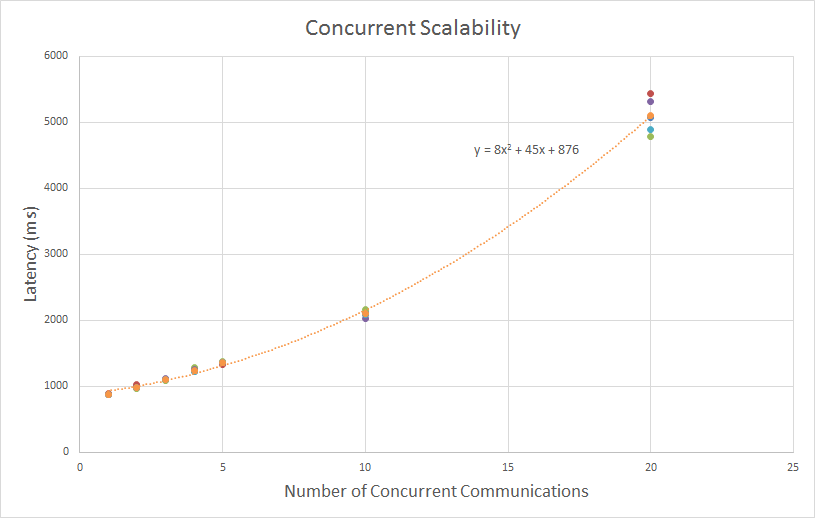
\includegraphics[width=0.7\textwidth,natwidth=815,natheight=518]{figures/concurrentsubmit.png}
\caption{Latency with Number of Concurrent Communications for Submit Protocol}
\label{fig:concurrentsubmit}
\end{figure}

Despite the polynomial growing trend, the protocol is still proved to be efficient under relatively small scale (less than 20 communications). The result shows that even when the message creator is communicating with 20 different couriers at the same time, the latency for running 100 times of protocol is still around 5 seconds (50 milliseconds for a single protocol run), considering the average latency for a single protocol run is 5.5 milliseconds (tested above), this result is fairly tolerable.

\pagebreak
\section{Transmit Protocol}
\subsection{Latency Test}
The definition of latency for Transmit Protocol is slightly different from Submit Protocol's. Referring to the protocol specification, Transmit Protocol requires only 2 messages, one forwarded from Courier to Bob, one replied from Bob to Courier. Here the latency is defined as the total time cost from the point that Courier initiates a connection, to the point that Courier receives the message 2 and finishes checking its validity.

Follow the same program settings of Submit Protocol, the latency tests for Transmit Protocol records the time cost for running 100, 200, 300, ..., 1000 times of the protocol. The message size is still 18 bytes.

\begin{figure}[h!]
\centering
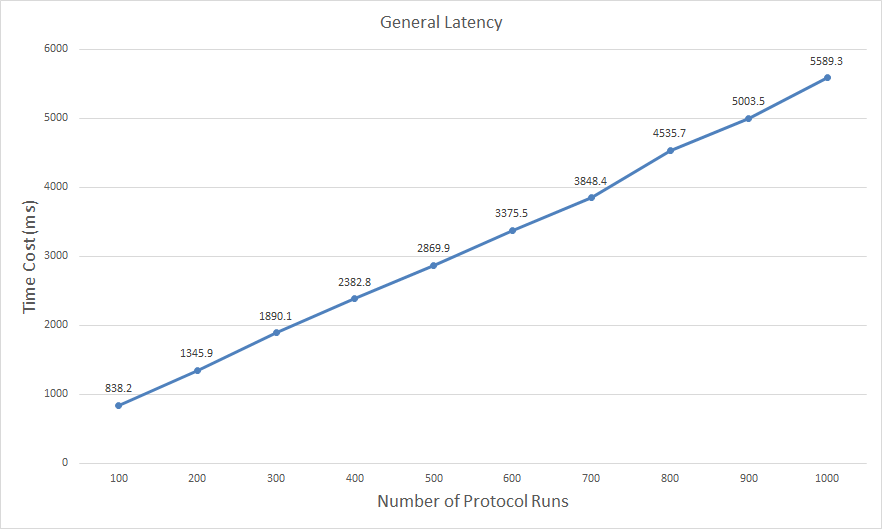
\includegraphics[width=0.7\textwidth,natwidth=882,natheight=529]{figures/latencytransmit.png}
\caption{General Latency Test of Transmit Protocol}
\label{fig:latencytransmit}
\end{figure}

Figure~\ref{fig:latencytransmit} shows the testing result. As expected, the outcome is quite similar to Submit Protocol, which appears to be linearly increasing. And even the average latency for each run of Transmit Protocol is same to Submit Protocol, which is given in figure~\ref{fig:averagelatencytransmit}. It can be observed that after doing Transmit Protocol many times, finally the average latency stabilized around 5.5 milliseconds. It proves the protocol is as efficient as Submit Protocol.

\begin{figure}[h!]
\centering
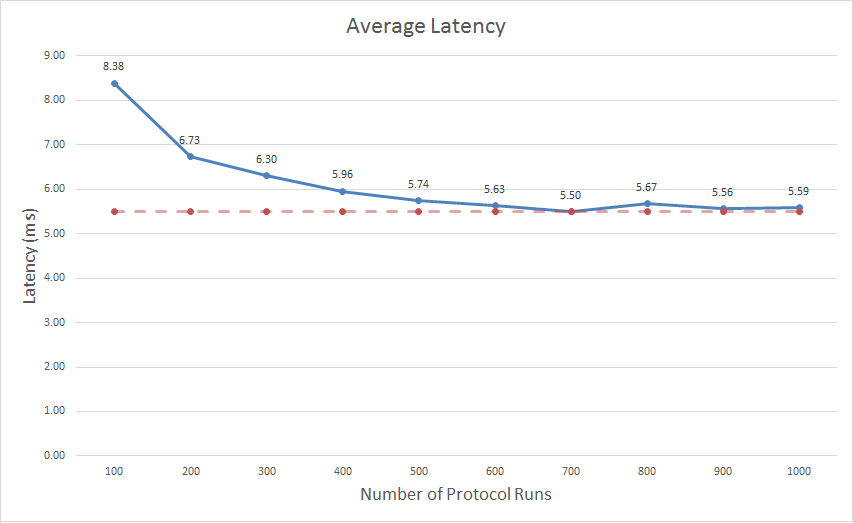
\includegraphics[width=0.7\textwidth,natwidth=853,natheight=523]{figures/averagelatencytransmit.png}
\caption{Average Latency of Transmit Protocol}
\label{fig:averagelatencytransmit}
\end{figure}

\subsection{Scalability Test}
In the scalability test of Transmit Protocol, besides testing under different scale of message size and number of concurrent communications, a new parameter is to be tested - number of messages. Their methodologies and analysis results will be given separately below.

\subsubsection{Scale of Message Size}
The methods and program settings used in this test is exactly the same with Submit Protocol, which is, a courier sends a message to Bob for 1000 times with different message size. The message sizes are 1 Byte, 10 Bytes, 100 Bytes, 1 KB, 2 KB, 3 KB, 4 KB, 5 KB and 10 KB respectively. The results are plotted in figure~\ref{fig:messagesizetransmit}, which indicates that the latency increase is fairly little comparing to the increase of message size. And it can be observed that the performance of Transmit Protocol when transmitting large messages is slightly better than Submit Protocol, it only takes 6 seconds to transmit a 10 KB message 1000 times, while it takes 6.2 seconds to submit it. 

\begin{figure}[h!]
\centering
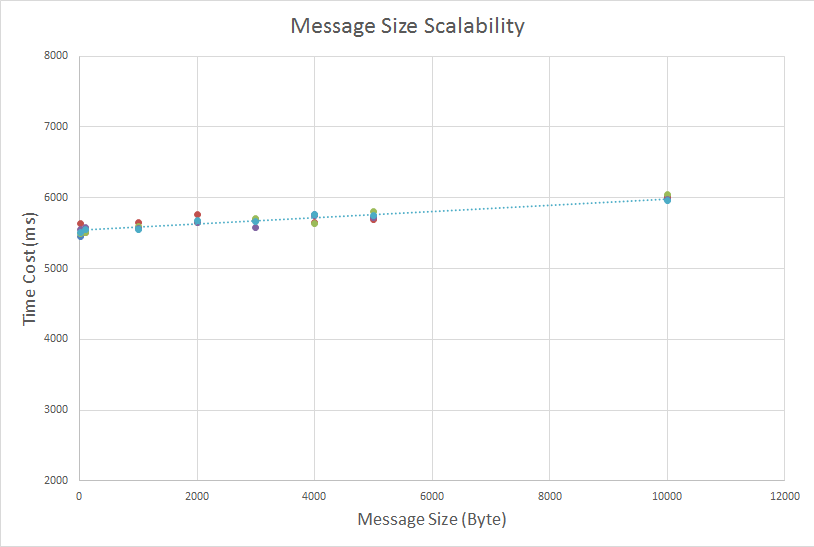
\includegraphics[width=0.7\textwidth,natwidth=814,natheight=547]{figures/messagesizetransmit.png}
\caption{Latency with Message Size for Transmit Protocol}
\label{fig:messagesizetransmit}
\end{figure}

The relationship between message size and effective throughput of Transmit Protocol is illustrated in figure~\ref{fig:effectivethroughputtransmit}. Similar to the Submit Protocol, the effective throughput has linear positive correlation with the message size. It means the larger the size of single message is, the more efficient of the protocol will be. And by observing figure~\ref{fig:effectivethroughputsubmit} and figure~\ref{fig:effectivethroughputtransmit}, we can conclude that overall, the efficiency of Transmit Protocol is slightly better than Submit Protocol because its latency is always less than Submit Protocol when they are tested under the same condition.

\begin{figure}[h!]
\centering
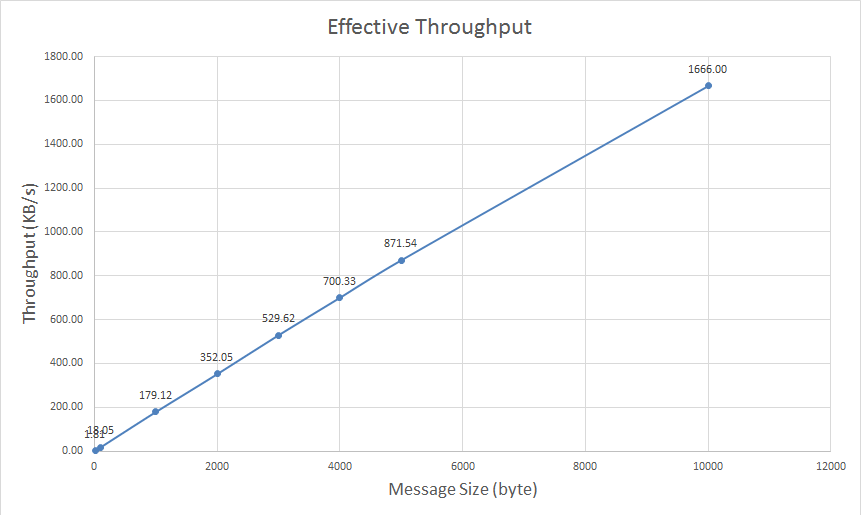
\includegraphics[width=0.7\textwidth,natwidth=861,natheight=515]{figures/effectivethroughputtransmit.png}
\caption{Effective Throughput with Message Size for Transmit Protocol}
\label{fig:effectivethroughputtransmit}
\end{figure}

\subsubsection{Scale of Concurrent Communication}
Same concurrency test is done to Transmit Protocol to reflect the practical scenario when a single message recipient (Bob) may receive messages from multiple couriers. The program settings are same to Submit Protocol: certain number of silent couriers keep communicating with Bob silently, while one noisy courier records the number of communication and yields the time cost. 

The testing result is shown in the figure~\ref{fig:concurrenttransmit}. The trend line of data samples is quite similar to the one of Submit Protocol, they both indicate a polynomial correlation. However, the growth rate of it in Transmit Protocol is much less than in Submit Protocol. We can find that when communicating with 20 couriers, Transmit Protocol takes only 3.2 seconds to complete 100 times of protocol, while Submit Protocol takes about 5 seconds. It means courier will be more efficient to transmit messages than to receive messages.

\begin{figure}[h!]
\centering
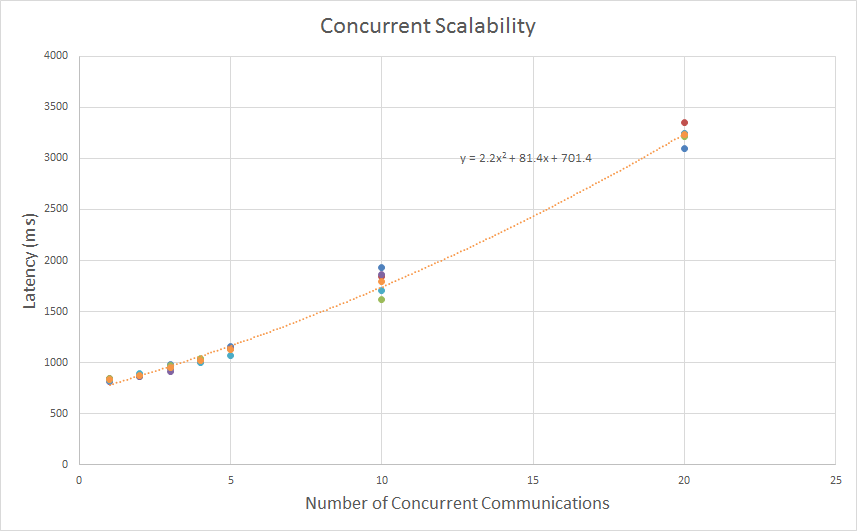
\includegraphics[width=0.7\textwidth,natwidth=857,natheight=531]{figures/concurrenttransmit.png}
\caption{Latency with Number of Concurrent Communications for Transmit Protocol}
\label{fig:concurrenttransmit}
\end{figure}

\subsubsection{Scale of Message Number}
This test simulates a common situation that a single Courier carries messages from several message creators and transmit it to the message recipient once for all. It is the most basic communication model in the system, so we are curious about how it performs in the actual implementation. Theoretically, the number of messages raises does not only lead to the increasing of message size, more extra checking processes are required as well. The test aims to find out how severe its influence will be.

This test measures the latency of total 100 Transmit Protocol runs with different number of messages transmitted. The number of messages are 1, 2, 3, 4, 5, 10, 20, and each message has size of 1 KB. Totally 5 tests are done and the average number of them is taken as the final outcome.

Figure~\ref{fig:messagenumbertransmit} shows the linear correlation of between number of messages and latency. It indicates that to sequentially complete 100 Transmit Protocols for a courier who carries 20 messages, it takes about 4 seconds in total, which means 40 milliseconds for every completion of the protocol. It is a great cost increase comparing to 5.5 ms, which is the average latency per protocol run. 

\begin{figure}[h!]
\centering
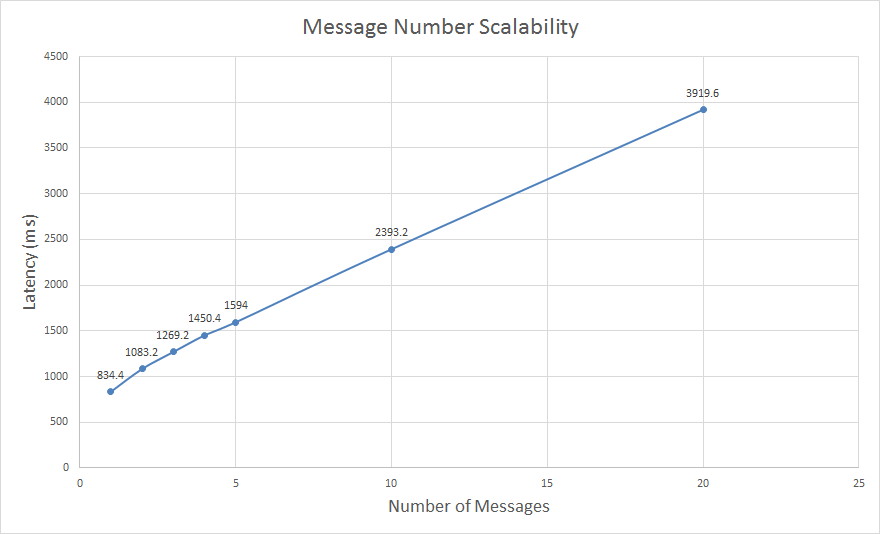
\includegraphics[width=0.7\textwidth,natwidth=880,natheight=534]{figures/messagenumbertransmit.png}
\caption{Latency with Number of Messages for Transmit Protocol}
\label{fig:messagenumbertransmit}
\end{figure}

Furthermore, the figure~\ref{fig:throughputcomparison} compares the efficiency difference between transmitting a large message as whole and chopping it into several pieces of smaller messages. The comparison takes several large size messages, and (1) transmits it as a whole, (2) transmits it as several 1 KB size smaller messages, and show their effective throughput respectively. The result conveyed by the figure is absolutely clear: no matter what the total message size is, transmitting it as a large message has nearly twice the throughput than chopping it up.

\begin{figure}[h!]
\centering
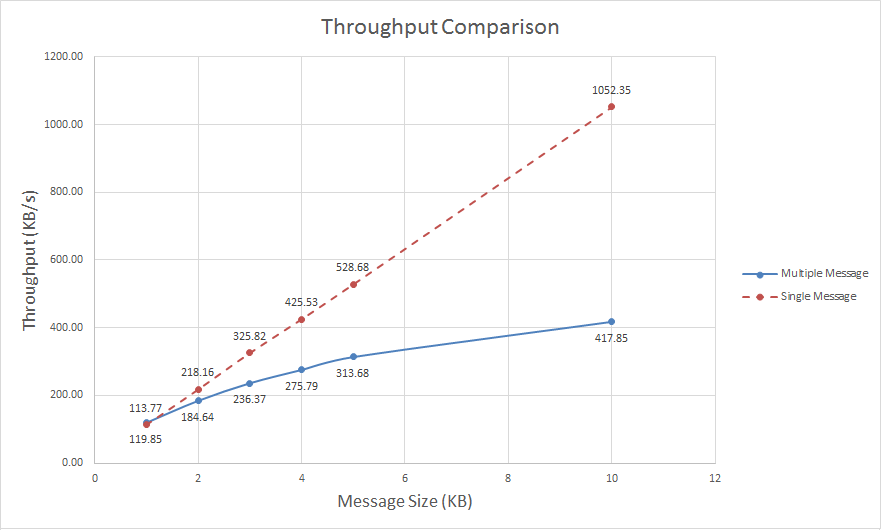
\includegraphics[width=0.7\textwidth,natwidth=881,natheight=530]{figures/throughputcomparison.png}
\caption{A Large Message or Several Small Messages?}
\label{fig:throughputcomparison}
\end{figure}

Conclusions drawn from both figure~\ref{fig:messagenumbertransmit} and figure~\ref{fig:throughputcomparison} indicate that transmitting large number of messages in a single Transmit Protocol is very time consuming. Thus when Alice sending a large message to Bob, it is recommended to send it as a whole for the efficiency concern.

\section{Summary}
In this chapter, mainly two kinds of tests are applied to both Submit Protocol and Transmit Protocol respectively - latency test and scalability test. Latency test evaluates the time cost for completing a protocol under a relatively low workload, while scalability test reveals the behaviour of both protocols when the system scale dramatically grows. The testing results prove that both Submit and Transmit Protocol are very efficient, every single run of protocol in low-workload situation takes only 5.5 milliseconds for both of the protocols. And in terms of scalability, both sub-protocols behave surprisingly the same. Firstly they are both not sensitive to the increasing of message sizes, and their latencies have polynomial correlation with the number of concurrent communications. Besides, through the analysis of relation between latency and number of message sizes, it has been emphasized that sending a large message as whole is far better than sending it as several pieces of smaller messages.
\chapter{Conclusion and Future Work}
\section{Conclusion}
The recently introduced Delay-Tolerant Network architecture assembles networks with different latencies, bandwith limitations or node longevities together and makes the interoperation between them achievable. Although DTN's high level security issues have been analysed and implemented in many publications, there is no a proper protocol specifically focusing on its courier-dependent custody transferring. Two of the related security protocols - Bundle Security Protocol and DTN Anonymity and Secure Architecture, have been examined and discussed, consequently, it has been shown that there are still some improvements to be made.

Then a new security protocol specifically designed for courier-dependent communication is created, named Courier-Dependent Security Protocol (CDSP). It has following main security achievements - authentication of originator and recipient, authenticity of origin of the message, confidentiality of the message content and deniability for originator and recipient, and the time efficiency of the protocol is raised to a high priority. To show the protocol, firstly the whole system that the protocol will be working in is fully described. Then is the protocol specification, specifies the detailed procedure of CDSP step by step. The last part of the protocol illustration summaries all security properties of CDSP, showing its capability and then proves every one of those properties. 

After CDSP has been thoroughly described, a concrete implementation of this protocol is developed in JAVA. The program mainly consists of a core library which provides all essential functions to run CDSP and a runnable application uses the core library. The core library is designed with emphasized extensibility and reusability, thus it can be easily modified and extended after the prototype released. The program architecture is illustrated by understandable figures and its security-related designs are fully documented afterwards.

Finally the application is tested for performance evaluation. Two main aspects - transferring latency and scalability have been taken into account, and some interesting conclusions of the protocol behaviour have been made.

\section{Discussion and Future Work}
The most obvious defect of this protocol system is that the success delivery of messages is never guaranteed by courier. Due to the efficiency and simplicity concerns, couriers are never required to authenticate to message creator, which means any entity can claim itself as courier and get the data. It leads to the problem that message creator will never know whether her message has been submitted to the real courier, neither will her know whether her message will eventually be delivered to the recipient. This kind of uncertainty can be problematic in some scenarios where the success delivery guarantee is strongly demanded - like transmitting military intelligence. One potential solution can reduce the extend of its uncertainty by forcing couriers to authenticated to message creator before they run Submit Protocol. It ensures only authorized couriers can successfully get data from message creator, and assume only well behaved couriers can get authorized, the probability of success delivery will definitely be increased. Furthermore, if any message is lost by a courier, later it will be very easy to trace back to the troublemaker. Nevertheless, the drawback of it is also non-negligible. Firstly it increases the overhead for key distribution and management as not only end users possess unique key pairs but also every authorized couriers. Secondly it burdens the running of CDSP as mutual authentication is needed when both Submit and Transmit Protocols. As a consequence, in the future implementation, it would be reasonable to provide both two sets of protocols in the application and leave it for users to choose which one to run based on the specific circumstances.

Another imperfection in the protocol design is that: after running the protocol, message originator can not fully deny sending a message to the recipient. As stated in the protocol property specification, this compromise is made to minimize the computational complexity while running the protocol as non-interactive deniable authentication is computational consuming. So, in the future implementation, it is also expected that user can choose which deniable authentication method to use based on the specific circumstances.

Besides, the protocol specification does not cover the corresponding schemes for key distribution, key management and key revocation, instead, they are assumed to be taken care of before running the protocol. Although making such minimum assumptions about the requirements makes the protocol as generic as possible, however, it may reduce the consistency of the whole system. Thus we hope that the best fitted key manipulation schemes can be created for CDSP protocol in the future revised designs.

Also it will be plausible if application can be developed in portable devices, so that tests and evaluations can be done on the portable devices as well. It obviously is more close to the real scenario where only portable devices will be used as couriers in the protocol, and with the extensible and reusable core library developed, it will not be a too time-consuming task.

Finally the efficiency of the protocol always need to be improved as it is one of the main requirement of the protocol design. Efficiency improvement could be accomplished by exploring some more newly invented efficient cryptographic operations and substitute the less efficient ones, or by further revising the code of the implementation.

%now enable appendix numbering format and include any appendices
\appendix
%\chapter{User Manual}
To start a protocol using this application involves 3 basic steps - (1) user chooses a specific protocol role. (2) user inputs the information related to the selected protocol role. (3) user starts the protocol. Below is a snapshot of current GUI of the application, it basically consists of 4 main panels:

\begin{figure}[h!]
\centering
\includegraphics[width=\textwidth,natwidth=818,natheight=722]{figures/guiall.png}
\caption{GUI Overview}
\end{figure}

\begin{itemize}
\item \textbf{Protocol Entity}\\
It is on the very top. It provides 4 roles (as mentioned above) to be chosen for the user. Because every device runs this protocol must be one of those four roles, it is essential that user specifies a role in this panel before start running the protocol.
\item \textbf{Entity Identity}\\
It locates on the left. Here user specifies the information about the host device and the destination device, such like IDs, and IP addresses.
\item \textbf{File Paths}\\
It locates on the right. Here user manages all the disk files that are related to the running of the protocol. Presumably, many important information like public keys, private keys and messages are all files in the device's disk, user has to specify those files' paths before running the protocol.
\item \textbf{Console}\\
It is at the bottom. Here provides buttons for user to start and stop the protocol, and it displays information about the running protocol in a information board.
\end{itemize}

\section{Run Submit Protocol}
It requires at least 2 devices to run this protocol, we call them $ D_0 $ and $ D_1 $. Assume $ D_0 $ is entity Alice, who possesses a message and wants to send it to Bob. Assume $ D_1 $ is entity Courier, who is able to carry the message and transmit it to Bob. To run the protocol successfully, it should be done by the following procedure:
\begin{enumerate}
\item $ D_0 $ starts the application.

\item $ D_0 $ user selects ``DataCreator" in the Protocol Entity panel.

\item $ D_0 $ user specifies the entity ID, local address and listening port (9888 by default) by filling the corresponding textfields in Entity Identity panel.

\item $ D_0 $ user adds destination entity's public key into its public key list.\\
There are two ways to add an new entry to the public key repository:
 \begin{enumerate}
 \item Adding through application: input the ID of the public key holder and the path of public key file by filling the textfields in the Public Key panel. Then click Add button. The (ID, path) pair will then appear in the public key list. This effect is temporary, the pair will disappear in the next launch.
 \item Adding through configuration file: by default, when application is launched, it will import all (ID, path) pairs from a file named PublicKeys in the current directory. User can appending a new line to PublicKeys file to add a new pair. The format is ID;Path, e.g. ``Alice;/publickeys/alice.pk". This effect will take place since next launch of the application.
 \end{enumerate}

\item $ D_0 $ user specifies its private key by filling the textfield with the private key file.

\item $ D_0 $ user specifies recipient entity's ID by filling the textfield in the Data to Send panel.

\item $ D_0 $ user specifies the file that contains the message needs to be sent by filling the file path in the corresponding textfield.

\item $ D_0 $ user click Start button in the Console panel. The running progress of the protocol will be displayed in the information board in the Console panel.

\item $ D_1 $ starts the application.

\item $ D_1 $ user selects ``CourierReceiver" in the Protocol Entity panel.

\item $ D_1 $ user specifies its own entity ID by filling the textfield in Entitiy Identity panel.

\item $ D_1 $ user specifies the ID of the entity he wants to contact (here $ D_0 $'s ID), together with its address and port number by filling corresponding textfields in the rest of Entity Identity panel.

\item $ D_1 $ user add the public key of the entity he wants to contact into the public key list. The way of doing that has been introduced in step 4.

\item $ D_1 $ user click the Start button in the Console panel. The running progress of the protocol will be displayed in the information board in the Console panel.
\end{enumerate}
Below figures show snapshot of two applications successfully running Submit Protocol. After application consoles on both devices pops ``process finish" successfully, the message of $ D_0 $ has been submitted to the $ D_1 $, and is stored in the file named by the message recipient's ID. If $ D_1 $ gathers messages from multiple devices, all messages to the same recipient will be accumulated in the same file.

\begin{figure}[!h]
 \centering
 \begin{subfigure}[b]{0.49\textwidth}
  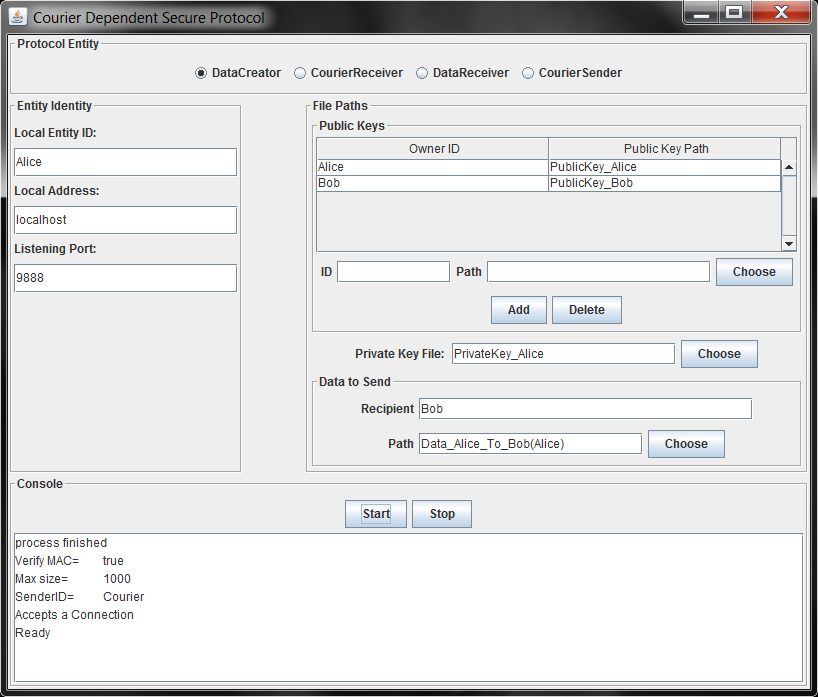
\includegraphics[width=\textwidth,natwidth=818,natheight=697]{figures/GUIdatacreator.png}
  \caption{DataCreator}
 \end{subfigure}
 \begin{subfigure}[b]{0.49\textwidth}
  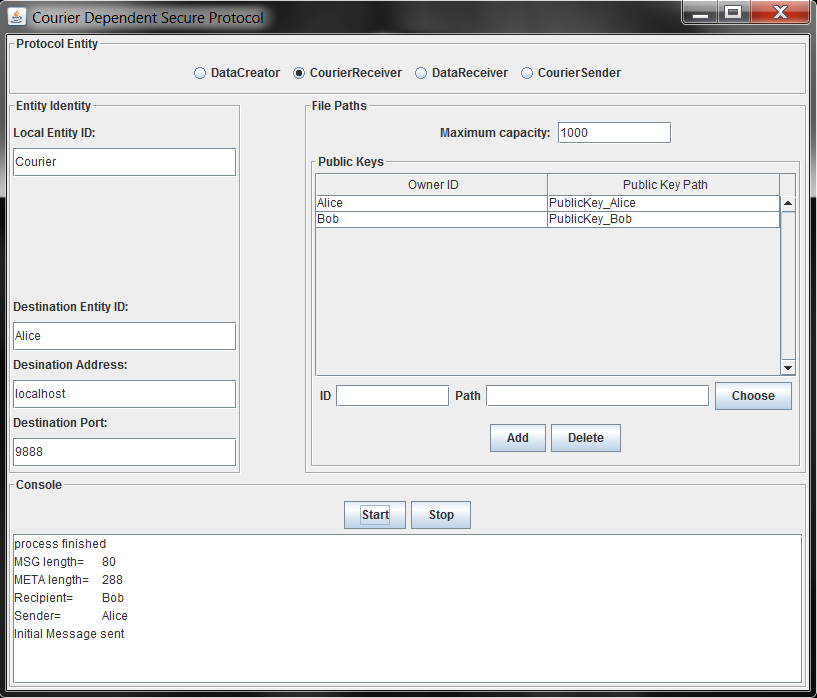
\includegraphics[width=\textwidth,natwidth=817,natheight=698]{figures/GUIcourierreceiver.png}
  \caption{CourierReceiver}
 \end{subfigure}
 \caption{Running Submit Protocol} 
\end{figure}

\section{Run Transmit Protocol}
It requires at least 2 devices to run this protocol, we call them $ D_1 $ and $ D_2 $. Assume $ D_1 $ is entity Courier, who possesses an encrypted message from Alice and wants to send it to Bob. Assume $ D_2 $ is entity Bob, who waits to receive message from Alice. The running procedure of Transmit Protocol is:

\begin{enumerate}
\item $ D_2 $ starts the application.

\item $ D_2 $ user selects ``DataReceiver" in the Protocol Entity panel.

\item $ D_2 $ user specifies the entity ID, local address and listening port (8888 by default) by filling the corresponding textfields in Entity Identity panel.

\item $ D_2 $ user adds destination entity's public key into its public key list. The way of doing that has been introduced in the step 4 of running Submit Protocol.

\item $ D_2 $ user specifies its private key by filling the textfield with the private key file.

\item $ D_2 $ user click Start button in the Console panel. The running progress of the protocol will be displayed in the information board in the Console panel.

\item $ D_1 $ starts the application.

\item $ D_1 $ user selects ``CourierSender" in the Protocol Entity panel.

\item $ D_1 $ user specifies its own entity ID by filling the textfield in Entitiy Identity panel.

\item $ D_1 $ user specifies the ID of the entity he wants to contact (here $ D_2 $'s ID), together with its address and port number by filling corresponding textfields in the rest of Entity Identity panel.

\item $ D_1 $ user add the public key of the entity he wants to contact into the public key list. The way of doing that has been introduced in step 4.

\item $ D_1 $ user specifies the file that contains the data needs to be sent, by filling the file path in the corresponding textfield in Data to Send panel.

\item $ D_1 $ user click the Start button in the Console panel. The running progress of the protocol will be displayed in the information board in the Console panel.
\end{enumerate}
Below figures show snapshot of two applications successfully running Transmit Protocol. After application consoles on both devices pops ``process finish" successfully, the data carried by $ D_1 $ has been transmitted to $ D_2 $. If the authenticity of the data is successfully verified, $ D_2 $ will print the message content out in the information board. If the data contains messages from multiple senders, they will be verified and printed one by one so that user knows which messages have been discarded.

\begin{figure}[!h]
 \centering
 \begin{subfigure}[b]{0.49\textwidth}
  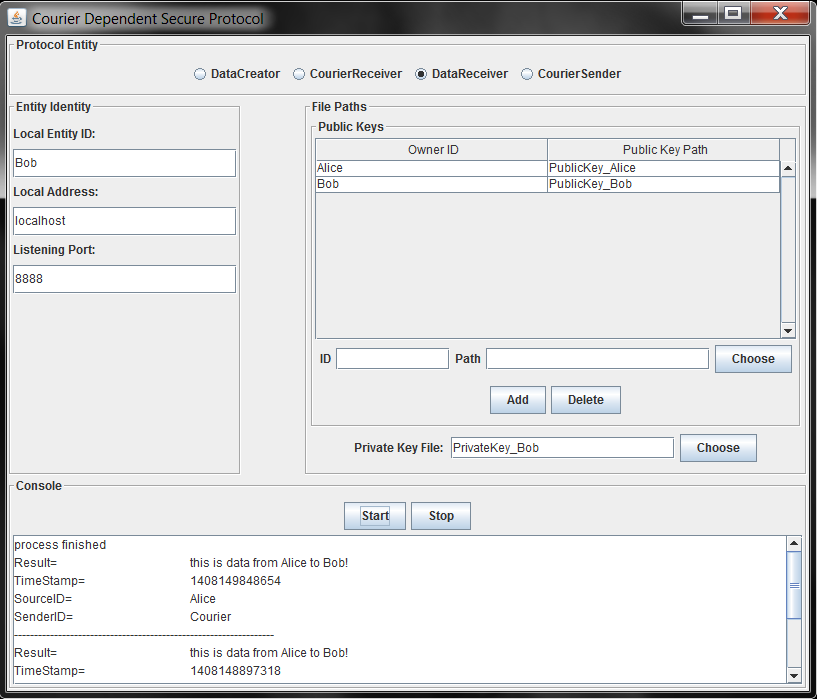
\includegraphics[width=\textwidth,natwidth=818,natheight=697]{figures/GUIdatareceiver.png}
  \caption{DataReceiver}
 \end{subfigure}
 \begin{subfigure}[b]{0.49\textwidth}
  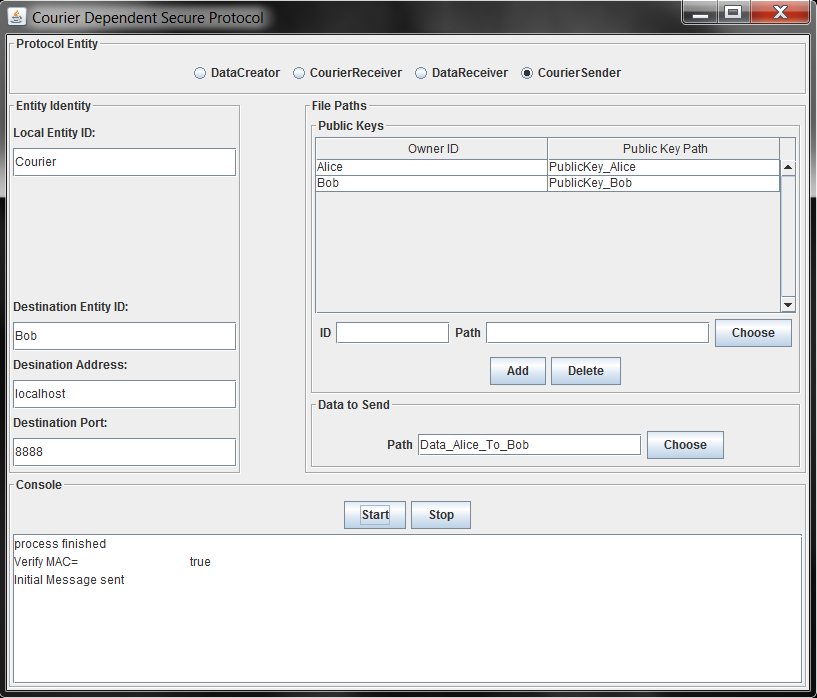
\includegraphics[width=\textwidth,natwidth=817,natheight=698]{figures/GUIcouriersender.png}
  \caption{CourierSender}
 \end{subfigure}
 \caption{Running Transmit Protocol} 
\end{figure}
%\chapter{Sample Title}

Lorem ipsum dolor sit amet, consectetur adipiscing elit, sed do eiusmod tempor incididunt ut labore et dolore magna aliqua. Ut enim ad minim veniam, quis nostrud exercitation ullamco laboris nisi ut aliquip ex ea commodo consequat. Duis aute irure dolor in reprehenderit in voluptate velit esse cillum dolore eu fugiat nulla pariatur. Excepteur sint occaecat cupidatat non proident, sunt in culpa qui officia deserunt mollit anim id est laborum.

%next line adds the Bibliography to the contents page
\addcontentsline{toc}{chapter}{Bibliography}
%uncomment next line to change bibliography name to references
\renewcommand{\bibname}{References}
\bibliography{refs}        %use a bibtex bibliography file refs.bib
\bibliographystyle{plain}  %use the plain bibliography style

\end{document}

